\documentclass[12pt]{report}
\usepackage[print,nopanel]{pdfscreen}
%\begin{print}
\usepackage{lipsum}% http://ctan.org/pkg/lipsum
\usepackage{titletoc}% http://ctan.org/pkg/titletoc
%\section{type}
%\usepackage{sagetex}

\usepackage{listings}

\usepackage{lastpage}
\usepackage{macro/macro}
\usepackage{float}
\usepackage{fancyhdr}
\usepackage{verbatim}
\usepackage[Glenn]{fncychap}
\lhead{\bfseries OpenSCAD's Customizer}
\usepackage[left=2.5cm, right=1.5cm, top=1.5cm, bottom=1.5cm]{geometry}
\pagestyle{fancy}
%\end{print}
\margins{2.5cm}{1.5cm}{1.5cm}{1.5cm}
\begin{screen}

\renewcommand{\encodingdefault}{T1}
\usepackage{setspace}
\linespread{1.5}
\renewcommand{\rmdefault}{ptm}
\end{screen}
\screensize{8cm}{9cm}
\overlay{overlay8.pdf}
\usepackage{graphicx}

\begin{document}
\newcommand{\centertext}[1]{\begin{center}\textbf{#1}\end{center}}
\newcommand{\student}{\vskip 2.5cm}
\newcommand{\supervisor}{\vskip 2cm}
\newcommand{\stamp}{\vskip 2.5cm}
\newcommand{\HRule}{\rule{\linewidth}{0.5mm}}
\newcommand{\projecttitle}{ \fontsize{24}{25}\selectfont \bf{Multi-Threaded Geometric Rendering}}
\newcommand{\tab}[1]{\hspace{.4\textwidth}\rlap{#1}}
\newcommand{\itab}[1]{\hspace{.05\textwidth}\rlap{#1}}
\newcommand{\logo}[1]{\includegraphics[scale=0.16]{#1}}
\newcommand{\submitted}{
\vskip 0.2in
\textnormal{ {\fontsize{14}{16}\selectfont \textbf{Project Report}} \\
	{\fontsize{12}{13}\selectfont of Major Project}\\
}
\vskip 0.2in

\textnormal{
 {\fontsize{14}{16}\selectfont \textbf{Bachelor of Technology}\\}
 {\fontsize{16}{17}\selectfont  (Computer Science and Engineering)\\}
}
\vskip 4cm
%\logo{images/gne.png}
%\image{0.7}{images/gne.png}{}

\includegraphics[width=7cm]{images/gne.png}
\vskip 2cm
\begin{minipage}{0.4\textwidth}
\begin{flushleft} \large
{Submitted by:}\\
\textnormal{{\fontsize{12}{13}\selectfont Amarjeet Singh Kapoor\\ D4CSE 2013-17 \\135005\\1311017 \\}} % Your name
\end{flushleft}
\end{minipage}
~
\begin{minipage}{0.4\textwidth}
\begin{flushright}
\textnormal{ \\
	 {\fontsize{12}{13}\selectfont Govind Sharma\\ D4CSE 2013-17 \\135026\\1311053\\}} % Supervisor's Name
\end{flushright}
\end{minipage}\\[1.5cm]
\HRule \\[0.4cm]

\textnormal{
Guru Nanak Dev Engineering College \\
Ludhiana 141006}
}


\newcommand{\pagetitle}{\begin{center}
\projecttitle
\Large\textbf{}\\
\submitted
\vskip 1cm

\end{center}}
\newcommand{\openoffice}{\textbf{OpenOffice}}
\newcommand{\frontmatter}[1]{\begin{Large} \textbf{#1} \end{Large}}
\newcommand{\ppttitle}{\begin{center}
\end{center}}

\begin{screen}
\ppttitle
\end{screen}
\footskip 0.7cm
\thispagestyle{empty} 
\pagetitle
\newpage
\pagenumbering{Roman}
\cfoot{\thepage}

\begin{Large}
\centertext{Abstract}
\end{Large}


User Interface for Customizing Models in OpenSCAD is the project that I worked upon for my 6-month training and also as Google summer of code project. It is under the umbrella organization of BRL-CAD. OpenSCAD is an open source organization that serves a free software to create solid 3d CAD objects. OpenSCAD has in a way redefined how easy 3D modeling can be. But the Wikipedia article on OpenSCAD says that it is a non-interactive modeler, but rather a 3D compiler based on a textual description language. Pay attention to the above line, it’s primarily what I’ll be talking about.

What the guys over at Wikipedia said is true but their version of the truth needs a little filtration (rather trimming). OpenSCAD’s way of customization is interactive, just not through a graphical interface. And this contingency makes the whole 3D modeling thing a little less easy than it can be. But all of that is about to change.

Solid 3D modeling. That sounds like some serious business. But it’s just an awesome tool for making models pertaining to many uses (mostly 3D printing). And 3D printing as we can all agree upon is cool. 3D models can be created by anyone using OpenSCAD. OpenSCAD is as much for designers as it is for you and me. What else can most people agree upon apart from the fact that solid 3D modeling is cool? A graphical interface is simpler and more intuitive to use. There is a general aversion for typing commands in order to get things done. Simply put, more people have an inclination towards GUI.

This is something that OpenSCAD lacked. But the benevolent folks at Thingiverse.com found a way to help out the demographic intersection of GUI lovers and OpenSCAD users. The website provides an easy to use interface to customize models of OpenSCAD. All one needs to do is upload the OpenSCAD file. After uploading the file, what you’ll see can only be described as being magic. I’m kidding, it’s just very useful is all. The OpenSCAD’s script is used to make a form containing slide bars, text boxes, combo boxes, labels, etc all for the singular purpose of customizing models.

My project was to include similar functionality into OpenSCAD itself. Constantly having to upload files created in one software (OpenSCAD) to a website in order to customize your models can get a little problematic as one is uploading scripts without being able to confirm how the script will translate into a form on the site. Wouldn’t it be great if everything is at one place, the original place: OpenSCAD? Of course, it would.

My project intends to define a user interface to customize models interactively instead of having to modify them manually. It will enable the user to create the templates for a given model which can further be changed as per user’s requirements.

This project will allow the modelers to create generic models (templates) which others can then customize to cater to their own use.
\newpage
\begin{Large}
\centertext{Acknowledgement}
\end{Large}

I, student of Guru Nanak Dev Engineering College, Ludhiana, have taken efforts in this project.
However, it would not have been possible without the kind support and help of many individuals
and organizations. I would like to extend my sincere thanks to all of them.\\

The author is highly grateful to Dr. M.S. Saini Director, Guru Nanak Dev Engineering College, Ludhiana for providing him with the opportunity to carry out his Six Weeks Training at
Testing and Consultancy Cell, Guru Nanak Dev Engineering College, Ludhiana.\\

The author would like to whole heartedly thank Dr. H.S. Rai Dean, Testing and Consultancy
Cell, Guru Nanak Dev Engineering College, Ludhiana who is a vast sea of knowledge and without whose constant and never ending support and motivation, it would never have been possible to complete the project and other assignments so efficiently and effectively.\\

Finally, I would thanks My Mentors at OpenSCAD organisation Marius Kintel and Torsten Paul. Without their encouragementand Guidence it would not have been possible to complete this project
in such an efficient manner.


\vskip 1.0cm 
\noindent Amarjeet Singh Kapoor


\newpage
\tableofcontents
\newpage
\listoffigures
\newpage
\listoftables
\newpage


\pagenumbering{arabic}
\cfoot{\thepage}

\newpage
\chapter{INTRODUCTION OF ORGANIZATION}
\begin{figure}[ht]
\centering
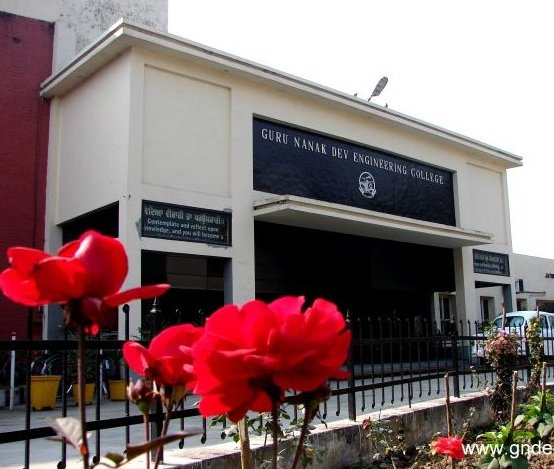
\includegraphics[scale=0.5]{images/gndec.jpg}
\caption{Guru Nanak Dev Engineering College}
\end{figure}
\hspace{-1.7em} I had my Six Month Industrial Training at TCC-Testing And Consultancy Cell, GNDEC Ludhiana. Guru Nanak Dev Engineering College was established by the Nankana
Sahib Education Trust Ludhiana. The Nankana Sahib Education Trust i.e NSET
was founded in memory of the most sacred temple of Sri Nankana Sahib, birth place
of Sri Guru Nanak Dev Ji. With the mission of Removal of Economic Backwardness
through Technology Shiromani Gurudwara Parbandhak Committee i.e SGPC started a
Poly technical was started in 1953 and Guru Nanak Dev Engineering College was established in 1956.\\


The main goal of this institute is:
\begin{itemize}
\item To build and promote teams of experts in the upcoming specialisations.
\item To promote quality research and undertake research projects keeping in view their
relevance to needs and requirements of technology in local industry.
\item To achieve total financial independence.
\item To start online transfer of knowledge in appropriate technology by means of establishing multipurpose resource centres.
\end{itemize}
\section{Testing and Consutancy Cell}

I had my Six Month Institutional Training at TCC i.e Testing And
Consultancy Cell,
GNDEC Ludhiana under the guidance of Dr. H.S.Rai Dean Testing and Consultancy Cell.
Testing and Consultancy Cell was established in the year 1979 with a basic aim to produce
quality service for technical problems at reasonable and affordable rates as a service to society
in general and Engineering fraternity in particular.\\
\begin{figure}[ht]
\centering
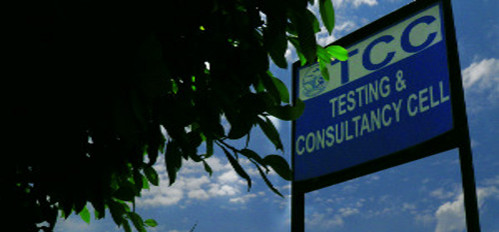
\includegraphics[scale=0.7]{images/aw.jpg}
\caption{Testing and Consultancy Cell}
\end{figure}
\hspace{-1.7em} 

Consultancy Services are being rendered by various Departments of the College to the
industry, Sate Government Departments and Entrepreneurs and are extended in the form of
expert advice in design, testing of materials \& equipment, technical surveys, technical audit,
calibration of instruments, preparation of technical feasibility reports etc.
This consultancy cell of the college has given a new dimension to the development
programmers of the College. Consultancy projects of over Rs. one crore are completed by the
Consultancy cell during financial year 2009-10. \\

Ours is a pioneer institute providing Consultancy Services in the States of Punjab, Haryana,
Himachal, J\&K and Rajasthan. Various Major Clients of the Consultancy Cell are as under:\\
\begin{itemize}
\item Northern Railway, Govt. of India
\item Indian Oil Corporation Ltd.
\item Larson \& Turbo.
\item Multi National Companies like AFCON \& PAULINGS.
\item Punjab Water Supply \& Sewage Board
\end{itemize}


\newpage


\chapter{Introduction To Project}
\section{Overview}

\begin{figure}[H] 
	\centering 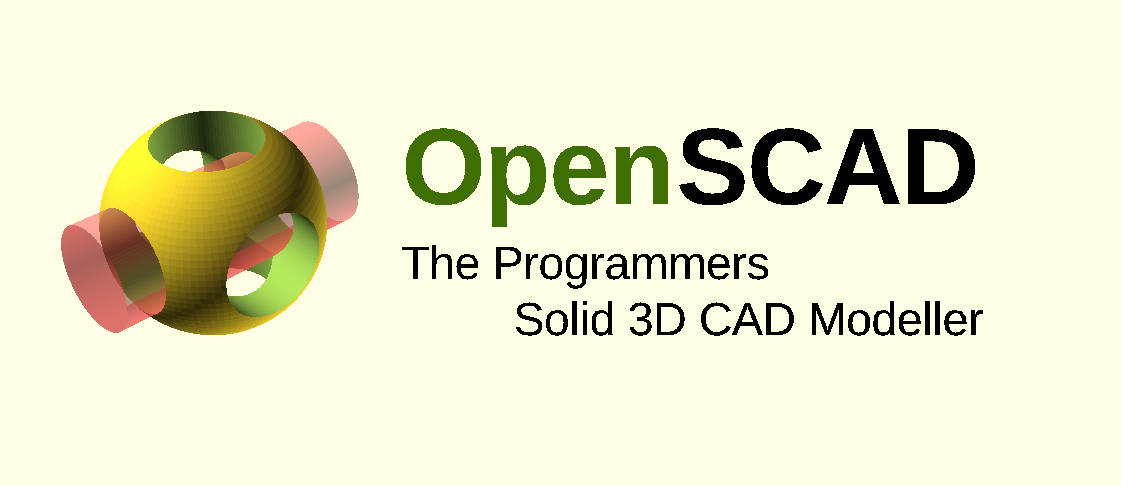
\includegraphics[scale=0.31]{images/openscad.png}
	\caption{OpenSCAD's logo}
	\label{fig:openscadlogo}
\end{figure}

User Interface for Customizing Models in OpenSCAD is the project that I worked upon for my 6 month training. It is under the umbrella organization of BRL-CAD. OpenSCAD is a free and Open source software application for creating solid 3D CAD objects. It is a script only based modeller, with a specific description language. Parts cannot be selected or modified by mouse in the 3D view. An OpenSCAD script specifies geometric primitives and defines how they are modified and manipulated to render a 3D model. OpenSCAD is available for Windows, Linux and OS X. It does constructive solid geometry (CSG).

OpenSCAD has in a way redefined how easy 3D modeling can be. But the Wikipedia article on OpenSCAD says that it is a non interactive modeler, but rather a 3D compiler based on a textual description language. Pay attention to the above line, it’s primarily what I’ll be talking about.

Solid 3D modeling. That sounds like some serious business. But it’s just an awesome tool for making models pertaining to many uses (mostly 3D printing). And 3D printing as we can all agree upon is cool. 3D models can be created by anyone using OpenSCAD. OpenSCAD is as much for designers as it is for you and me. What else can most people agree upon apart from the fact that solid 3D modeling is cool? A graphical interface is simpler and more intuitive to use. There is a general aversion for typing commands in order to get things done. Simply put, more people have an inclination towards GUI.

This is something that OpenSCAD lacked. But the benevolent folks at Thingiverse.com found a way to help out the demographic intersection of GUI lovers and OpenSCAD users. The website provides an easy to use interface to customize models of OpenSCAD. All one needs to do is upload the OpenSCAD file. After uploading the file, what you’ll see can only be described as being magic. I’m kidding, it’s just very useful is all. The OpenSCAD’s script is used to make a form containing slide bars, text boxes, combo boxes, labels, etc all for the singular purpose of customizing models.

My project was to include similar functionality into OpenSCAD itself. Constantly having to upload files created in one software (OpenSCAD) to a website in order to customize your models can get a little problematic as one is uploading scripts without being able to confirm how the script will translate into a form on the site. Wouldn’t it be great if everything is at one place, the original place: OpenSCAD? Of course, it would.

My project intends to define a user interface to customize models interactively instead of having to modify them manually. It will enable the user to create the templates for a given model which can further be changed as per user’s requirements.

This project will allow the modelers to create generic models (templates) which others can then customize to cater to their own use.

This project is based on the User interface of OpenSCAD Software. The main idea of this project is to provide users with features to change certain variables or parameters in .scad file using form like interface which may include slide bar, check box, text box, ranges etc. so that we can visualize the changes in output on the basis of input side by side instead of manually changing different parameters. It will help the user able to create the templates for given model which can further be changed as per user's requirements. 

The core part of this project is implemented using C++, flex and bison and for GUI part Qt is used. Apart for that Make, qmake and cmake are used for making project and test cases.
Testing is done using the travis and ctest. Github is used to manage code and IRC to communicate with the mentors.
  
My training being not based on particular language or technology, different type of open-source softwares and technologies are 
used in this project and many during my training which are not used in this 
project like android, ejabberd (server bassed on erlang and XMPP protcol) for\emph{ sunehaG} and GRASS GIS, python, shell scripting for \emph{The Road Project}.

\section{The Existing System}
The only System exiting to solve above problem is Thingiverse's Customizer which allows you to design parametric objects that can be customized with an easy web interface. They currently support OpenSCAD designs. Just upload your OpenSCAD script to Thingiverse and then anyone can open it in Customizer and customize it. Also, if you tag your Thing with the "customizer" tag, then your Thing page will automatically display an Open In Customizer button as a shortcut. 

But there syntax is little messy as they use comments to generate customizer which also limits the useablitiy of the customizer. \\

{\bf {Limitations of previous system }}
\begin{itemize}
\item \emph{Not supported by OpenSCAD offically.}

\item Doesn't work in combination with OpenSCAD software

\item Works only in online mode

\item No Command-line Support 

\item Based upon string processing not on lexical anylises. 

\item No internal support.

\item Commplex work flow.

\item Scripts must have all the code they need in a single .scad file

\item You could only put one .scad file in your Thingiverse entry
\end{itemize}

\section{User Requirement Analysis}
User Requirements Analysis for a software system is a complete description of the requirements of the User. It includes functional Requirements
and Non-functional Requirements. Non-functional requirements are
requirements which impose constraints on the design or implementation.

 
{\bf Users of the System:}
    \begin{enumerate}
        \item Modeler: Modelers are the people how the code to create model theirs for their own use or for commercial use.
        \item Client: These are the people which will customize model to their need made by modelers before ordering or printing model themselves.
        \item Other Softwares: Many web Apps or other software using OpenSCAD as there Backend might need to interact with the customizer.
               
    \end{enumerate}

\subsection{Functional Requirements}
\begin{itemize}
    \item {\bf Syntax to generate a widget to modify parameter}: This means there should be a syntax which could be used to generate a different widget for a different type of parameters.
    The widgets that we intend to support are:
    \begin{enumerate}
        \item Spinbox
            \begin{enumerate}
                \item With Increment Size
                \item Without Increment Size
            \end{enumerate}
        \item Checkbox
        \item Slider
            \begin{enumerate}
                \item With Increment Size
                \item With Default Increment Size
            \end{enumerate}
        \item Textbox
        \item Special vector
        \item Combo Box
            \begin{enumerate}
                \item Simple
                \item Labeled
            \end{enumerate}
   
    \begin{table}[h]
        \centering
        \caption{Table to show the required support of widgets for different DataType}
        \begin{tabular}{ |c|c|c|c|c|c| }
            \hline
            & \multicolumn{5}{|c|}{Type of Widgets} \\
            \hline
            Type of Data&    Number&    String&    BOOL &Vector &Range     \\ [0.5ex]
            \hline
            SpinBox&Y&    -&    -&    -&    - \\ \hline
            ComboBox&    Y&    Y&    -&    -&    - \\ \hline
            Text&    Y&    Y&    -&    O&    - \\ \hline
            Slider&    Y&    -&    -&    -&    - \\ \hline
            Checkbox&    -&    -&    Y&    -&    - \\ [1ex]
            \hline
        \end{tabular}
        \label{table2}
    \end{table}
   
    \end{enumerate}
    \item {\bf Syntax to Describe parameter}:
        This means there should be a syntax which could be used to provide a description for the parameter.
    \item \textbf{Syntax to Group Parameter}:
        This means there should be a syntax which could be used to group the parameters into different groups or tab to easily manage Customizer and make customizer interface little simple.
    \item \textbf{Syntax to Hide parameters}
        This means there should be a syntax which could be used to Hiding certain parameters.
    \item \textbf{Syntax to make certain parameters Global}
        This means there should be a syntax which could be used to make certain parameters global i.e. they are present in each and every group.
    \item \textbf{Save the set of parameters in JSON file}:
    This feature means there should be a way a way that gives user the ability to save the value of the parameter and also we can apply them through the cmd-line and get the output.
   
    \item \textbf{Provide GUI to add Set of Parameters}
        This means there should be a way to store different set of parameters which represent different models from generic model.
    \end{itemize}
\subsection{Non-functional requirements}
\begin{enumerate}
    \item Extensible: It should be able to support future functional requirements
    \item Usability: Simple user interfaces that a layman can understand.
    \item Modular Structure: The software should have  structure. So, that different parts of software would be changed without affecting other parts.
 
\end{enumerate}


\section{Feasibility Study}
Feasibility study aims to uncover the strengths and weaknesses of 
a project. In its simplest term, the two criteria to judge feasibility 
are cost required and value to be attained. As such, a well-designed 
feasibility analysis should provide a historical background of the 
project, description of the project or service, details of the 
operations and management and legal requirements. Generally, feasibility 
analysis precedes technical development and project implementation. 
These are some feasibility factors by which we can determine that 
project is feasible or not:
\begin{itemize}
\item {\bf{Technical feasibility}}: Technological feasibility is carried 
out to determine whether the project has the capability, in terms of 
software, hardware, personnel to handle and fulfill the user requirements. This whole project is based on Open 
Source Environment and is part of a open souce software which would be deployed on any OS.

\item {\bf{Economic feasibility}}: In Economic feasibitly we 
determine whether the benefit is gain according to the cost invested 
to develop the project or not. If benefits outweigh costs, only then 
the decision is made to design and implement the system. It is 
important to identify cost and benefit factors, which can be categorized 
as follows:
\begin{enumerate}
\item Development costs.
\item Operating costs.
\end{enumerate}
OpenSCAD's customizer is also Economically feasible with as It could be developed and maintain with zero cost as It is supported by Open source community.
Plus This project is started with no intention of having any economic gain but still their are option of donations. 

\end{itemize}



\section{Objective of Project}

One of the primary benefits of OpenSCAD is the ability to design customizable content. These are designs which are parametrized using parameters or top-level variables.


Some projects utilize OpenSCAD's ability to customize designs as part of their web services.
e.g. 
\begin{enumerate}
	\item Thingiverse Customizer
	\item  Sculpteo Parametric Designs
	\item e-NABLE Handomatic.
\end{enumerate}


The goal of this project is two-fold:
\begin{enumerate}
	\item  Offer an auto-generated GUI associated with a customizable design, making it easier to both create and use such designs
	\item Offer an authoritative standard for how to specify meta-data to guide the generation of such a GUI.
	
\end{enumerate}

As a temporary measure, we're also planning to support the meta-data syntax used by Thingiverse, making it possible to use the thousands of customizable designs published there.


%The major Objectives of this project are:
%\begin{enumerate}
%	\item Syntax support for generation of customization form:
%	The customization form generated on Thingiverse is based on a certain syntax for both describing the elements in the form and providing a range of their values. In order to make this work in OpenSCAD as well, the same style of description and parametrization can be incorporated into OpenSCAD. Hence the user will be able to generate the customization form from within OpenSCAD by adding a few simple lines in the .scad file.
%	
%	Customization of the model from the form:
%	Once the form is ready, it must be able to customize the model as desired by the user. The changes made in the form should directly correspond to changes in the model itself.
%	Enhancing the UI for the customization form:
%	The customization form is there to make the whole customization thing easy. And that implies that the form itself should also be easy to use. And this can be achieved by having a good and simple look to the whole thing.
%	
%\end{enumerate}




\chapter{PROJECT DESIGN}

% 1Product perspective
%[2] Product functions
%[3] User characteristics
%[4] Constraints
%[5] Use Case Model/Flow Chart/DFDS
%[6] Specific Requirements

\section{Flowchart}
A flowchart is a type of diagram that represents an algorithm, work flow or process, showing the steps as boxes of various kinds, and their order by connecting them with arrows
and the flowchart \ref{fig:FD1} of customizer showing the flow of control and Data in the software.

\begin{figure}
	\centering 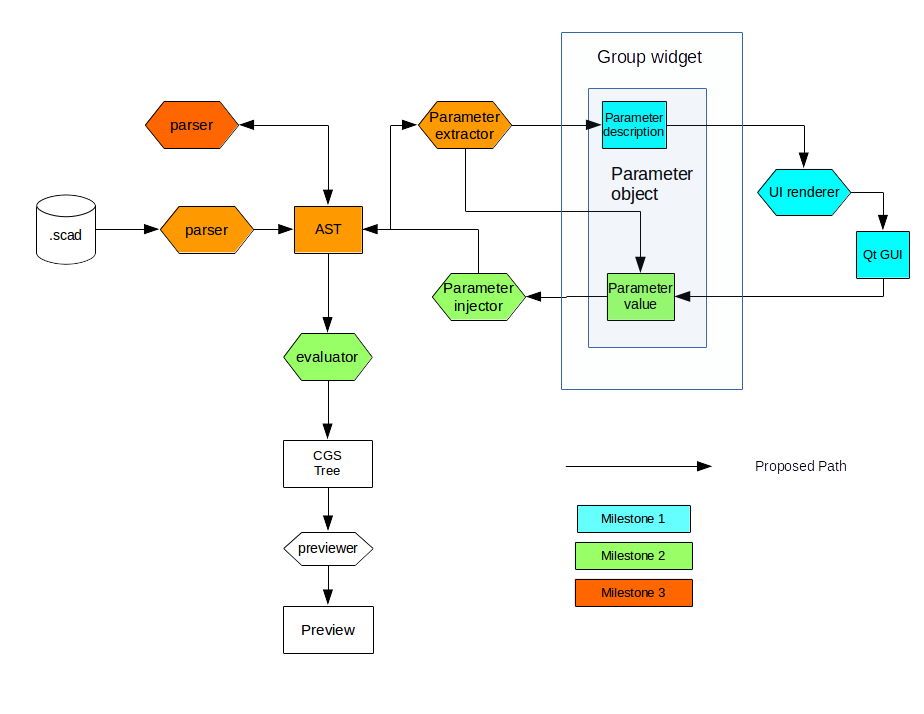
\includegraphics[width=\linewidth]{images/flowchart.png}
	\caption{Flowchart of Customizer}
	\label{fig:FD1}
\end{figure}

\subsection{Detailed Description}

The basic implementation of this project is almost done in form of prototype. There is need to modify the structure of the project. We have to divide the task into there parts:

\begin{enumerate}
	\item \textbf{Front end}
	It will deal with how the parameter will look to the user like in form of range or spinbox etc. This part will include two parts:
	\begin{enumerate}
		\item \textbf{Individual Parameter}
		This will define how individual parameters will look like
		\item \textbf{Container Widget}
		This will contain UI features common to all parameter. This widget will contain all parameter widget.
		
	\end{enumerate}
	
	\item \textbf{Back End}
	This will include the parser part that will create AST nodes and we can extract the parameters from the AST. we can use the single parser for the whole .scad file or separate parser for extracting the parameters with annotations.
	
	The Back-end part will also include the parameter extractor and injector or the injector can be included in parameter object which will serve as interface
	\item \textbf{Interface}
	This will include the parameter object which will serve as an interface between both Back end and Front end. Parameter object will contain information regarding each individual parameter like parameter name, default value, and information how this parameter will be displayed as widgets to the user. Parameter object could also include the method to inject the value of the individual parameter into the AST.
	
\end{enumerate}


\section{Dependency Graph}
A Dependency Graph is a graphical representation of the which module is dependent on which other modules. A Dependency Graph is often used as a preliminary step to creating an overview of the system. Dependency Graph also gives overview of how good is the design of the system.
OpenSCAD being were huge software it would be difficult to make the dependency graph of whole software. So, here is  Dependency Graph of Customizer is as following-:
\begin{enumerate}
\item \textbf{Dependency graph of Comment.h:} Figure \ref{fig:comment1} shows the modules on which the comment.h module is dependent.
\item \textbf{Caller graph of Comment.h:} Figure \ref{fig:comment} shows the modules that use the module comment.h.
\item \textbf{Caller graph of ParameterWidget.cc:} Figure \ref{fig:dependency} show the modules that uses the module ParameterWidget.h.
\end{enumerate}

\begin{figure}
	\centering
	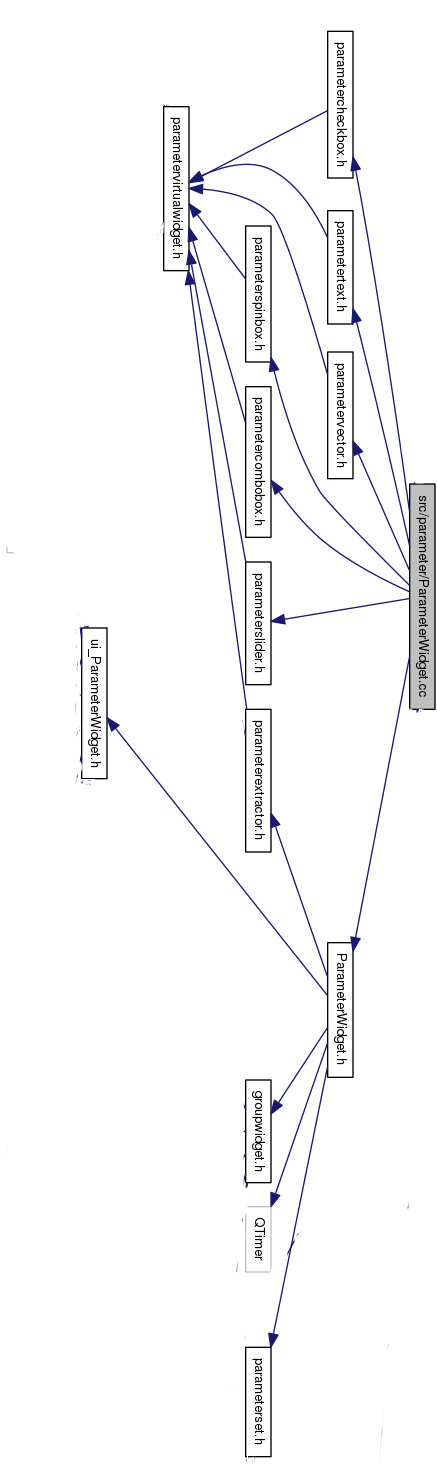
\includegraphics[width=0.7\linewidth,height=1.37\columnwidth]{images/dependene}
	\caption{ Dependency graph of Comment.h}
	\label{fig:dependency}
\end{figure}

\begin{figure}
\centering
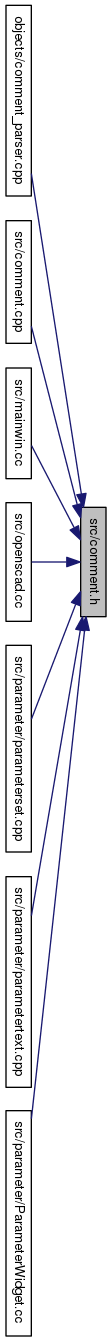
\includegraphics[width=0.25\linewidth,height=1.37\columnwidth]{images/comment}
\caption{Caller graph of Comment.h}
\label{fig:comment}
\end{figure}
\begin{figure}
\centering
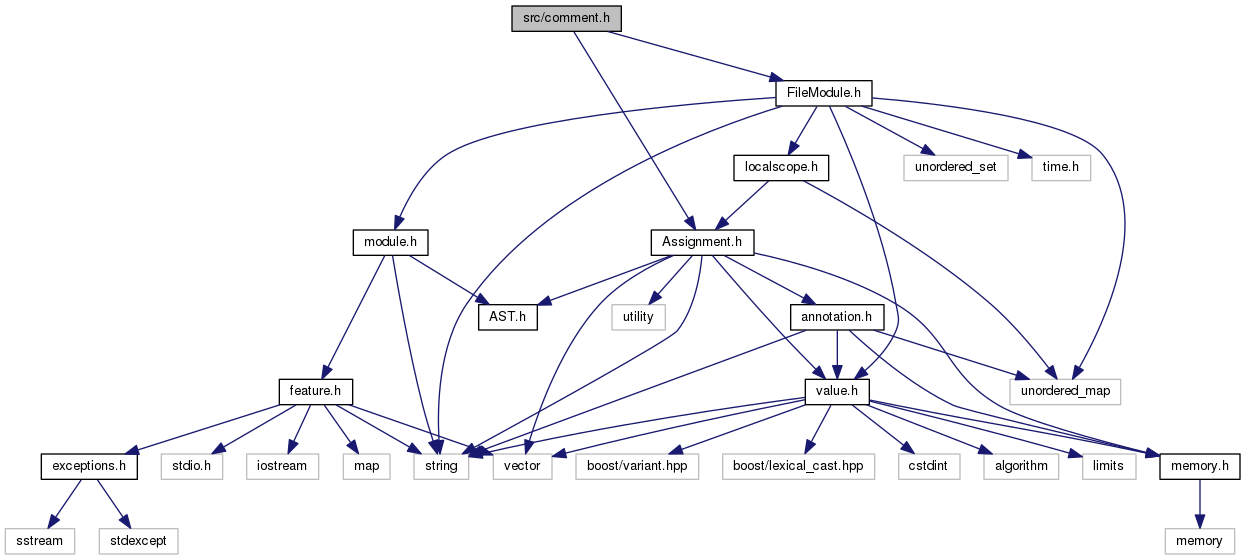
\includegraphics[width=\linewidth,height=1.35\columnwidth]{images/comment1}
\caption{Caller graph of ParameterWidget.cc}
\label{fig:comment1}
\end{figure}




\section{Class Diagrams}
Class Diagrams describe the static structure of the system. Following classes diagram represent the relationship between different classes in OpenSCAD and customizer:
\begin{enumerate}
	\item Figure \ref{fig:collaborative1} shows the class diagram of the ParameterWidgetVirtual class which is the basse class of all the Widget classes i.e ParameterCheckbox, ParameterVector,ParmeterSpinbox, ParameterComboBox,ParameterSlider, ParameterText.
	\item Figure \ref{fig:collaborative} shows the class diagram of the ParameterWidget class which is the main class for whole the Customizer GUI and also show how this class is related to various classes in custmoizer.
	
	\item Figure \ref{fig:classAnnotation__coll__graph}  shows the class diagram of the Annotation class which is the main node of the AST that support the customizer feature and also show how this class is related to various classes in the customizer.
\end{enumerate}
\begin{figure}
    \centering
    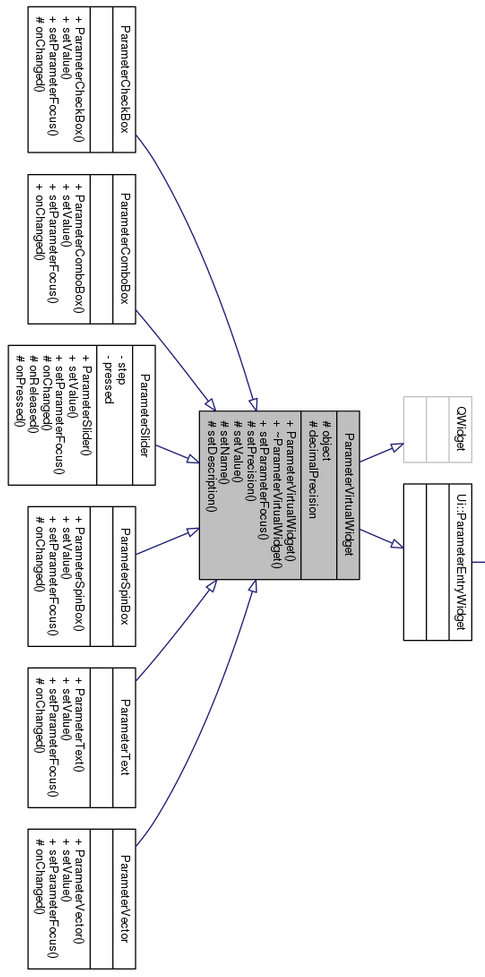
\includegraphics[width=0.5\linewidth,,height=1.38\columnwidth]{images/collaborative1}
    \caption{Class Diagram for Customizer (Part A) }
    \label{fig:collaborative1}
\end{figure}
\begin{figure}
    \centering
    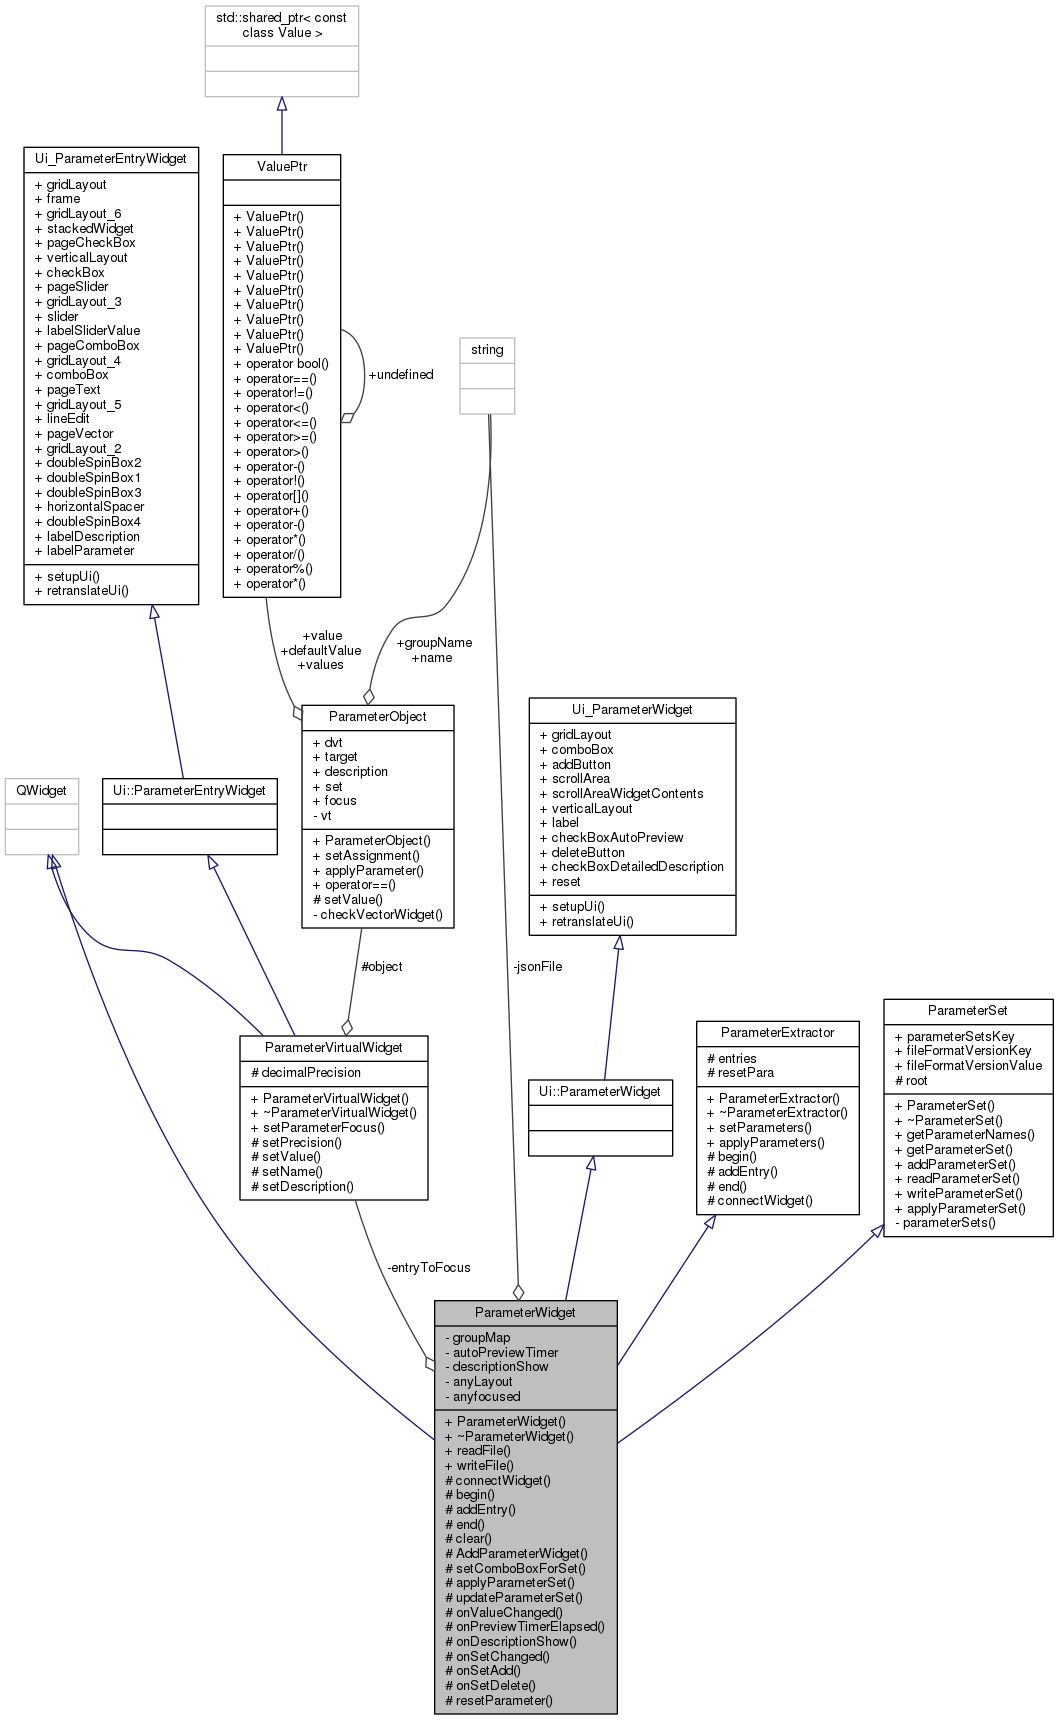
\includegraphics[scale=0.39]{images/collaborative}
    \caption{Class Diagram for Customizer (Part B)}
    \label{fig:collaborative}
\end{figure}
\begin{figure}
\centering
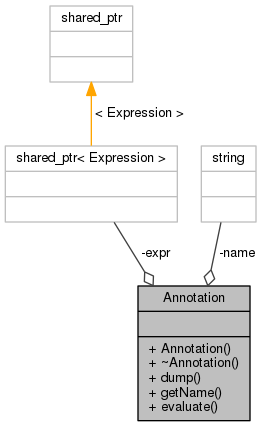
\includegraphics[width=0.4\linewidth]{images/classAnnotation__coll__graph}
\caption{Class Diagram for Annotation}
\label{fig:classAnnotation__coll__graph}
\end{figure}
\section{Dependencies}
Dependencies include softwares or framework that need to be installed for proper working of this software.

\emph{{\large There is no software dependencies to Install this software.}}

This software could be installed on any given list of operating system.

\begin{enumerate}
	\item Mac OS X
	\item Windows
	 \begin{enumerate} 
	 	\item XP or newer on x86 32/64 bit
	 \end{enumerate}
	\item Linux
	\begin{enumerate} 
		\item Debian 
		\item Ubuntu 
		\item Kubuntu
		\item Arch Linux
		\item openSUSE
		\item Fedora
	 \end{enumerate}
	\item BSD
	\begin{enumerate}
		\item NetBSD  $\geq 6.1$
		\item FreeBSD $\geq 10 $
		\item OpenBSD
	\end{enumerate}
\end{enumerate}	 
 

But If you want to build OpenSCAD this software from soucre code on \emph{any OS}, you need some libraries and tools. The version
numbers in brackets specify the versions which have been used for
development. Other versions may or may not work as well.

If you're using a newer version of Ubuntu, you can install these 
libraries from aptitude. If you're using Mac, or an older Linux/BSD, there 
are build scripts that download and compile the libraries from source. 
Follow the instructions for the platform you're compiling on below.

\begin{enumerate} 
	\item A C++ compiler supporting C++11
	
	\item Qt$  4.4 \rightarrow 5.x $ (http://qt.io/ )
	
	\item QScintilla2 $ (2.7 \rightarrow $)(http://www.riverbankcomputing.co.uk/software/qscintilla/)
	
	\item CGAL ($ 3.6 \rightarrow $) (http://www.cgal.org/)
	
	\item GMP (5.x) (http://www.gmplib.org/)
	
	\item MPFR (3.x)(http://www.mpfr.org/)
	
	\item cmake ($ 2.8 \rightarrow $, required by CGAL and the test framework))(http://www.cmake.org/)
	
	\item boost ($ 1.35 \rightarrow $) (http://www.boost.org/)
	
	\item OpenCSG ($ 1.3.2 \rightarrow $)(http://www.opencsg.org/)
	
	\item GLEW ($ 1.5.4 \rightarrow $)(http://glew.sourceforge.net/)
	
	\item Eigen (3.x)(http://eigen.tuxfamily.org/)
	
	\item glib2 (2.x)(https://developer.gnome.org/glib/)
	
	\item fontconfig ($ 2.10 \rightarrow  $)(http://fontconfig.org/)
	
	\item freetype2 ($ 2.4 \rightarrow  $)(http://freetype.org/)
	
	\item harfbuzz ($ 0.9.19 \rightarrow  $)(http://harfbuzz.org/)
	
	\item Bison ($ 2.4 \rightarrow $ )(http://www.gnu.org/software/bison/)
	
	\item Flex ($ 2.5.35 \rightarrow  $)(http://flex.sourceforge.net/)
	
	\item pkg-config ($ 0.26 \rightarrow $ )(http://www.freedesktop.org/wiki/Software/pkg-config/)
	
\end{enumerate}





\newpage
\chapter{DEVELOPMENT AND IMPLEMENTATION}
\section{C++}

\begin{figure}[h]
	\centering 
\includegraphics[scale=0.3]{images/c++.png}
	\caption{C++ Logo}
\end{figure}

C++ is a general-purpose programming language. It has imperative, object-oriented and generic programming features, while also providing facilities for low-level memory manipulation.

It was designed with a bias toward system programming and embedded, resource-constrained and large systems, with performance, efficiency and flexibility of use as its design highlights. C++ has also been found useful in many other contexts, with key strengths being software infrastructure and resource-constrained applications, including desktop applications, servers (e.g. e-commerce, web search or SQL servers), and performance-critical applications (e.g. telephone switches or space probes). C++ is a compiled language, with implementations of it available on many platforms and provided by various organizations, including the Free Software Foundation (FSF's GCC), LLVM, Microsoft, Intel and IBM.

C++ is standardized by the International Organization for Standardization (ISO), with the latest standard version ratified and published by ISO in December 2014 as ISO/IEC 14882:2014 (informally known as C++14). The C++ programming language was initially standardized in 1998 as ISO/IEC 14882:1998, which was then amended by the C++03, ISO/IEC 14882:2003, standard. The current C++14 standard supersedes these and C++11, with new features and an enlarged standard library. Before the initial standardization in 1998, C++ was developed by Bjarne Stroustrup at Bell Labs since 1979, as an extension of the C language as he wanted an efficient and flexible language similar to C, which also provided high-level features for program organization.

Many other programming languages have been influenced by C++, including C\#, D, Java, and newer versions of C (after 1998).

Features of Language:
\begin{enumerate}
	\item Object storage
	\begin{enumerate}
		\item Static storage duration objects
		\item Thread storage duration objects
		\item Automatic storage duration objects
		\item Dynamic storage duration objects
	\end{enumerate}
	\item Templates
	\item Objects
	\begin{enumerate}
		\item Encapsulation
		\item Inheritance
	\end{enumerate}
	\item Operators and operator overloading
	\item Polymorphism
	\begin{enumerate}
		\item Static polymorphism
		\item Dynamic polymorphism
		\begin{enumerate}
			\item Inheritance
			\item Virtual member functions
		\end{enumerate}
	\end{enumerate}
\item Lambda expressions
\item Exception handling
\end{enumerate}
\section{Flex}

Flex (fast lexical analyzer generator) is a free and open-source software alternative to lex. It is a computer program that generates lexical analyzers (also known as "scanners" or "lexers"). It is frequently used as the lex implementation together with Berkeley Yacc parser generator on BSD-derived operating systems (as both lex and yacc are part of POSIX), or together with GNU bison (a version of yacc) in *BSD ports and in GNU/Linux distributions. Unlike Bison, flex is not part of the GNU Project and is not released under the GNU Public License.

Flex was written in C by Vern Paxson around 1987. He was translating a Ratfor generator, which had been led by Jef Poskanzer

Input to Lex is divided into three sections with \%\% dividing the sections. Flex .l specification file:
\begin{verbatim}
	/*** Definition section ***/
	
	%%
	
	/*** Rules section ***/
	
	%%
	
	/*** C Code section ***/
\end{verbatim}

\section{Bison}

\begin{figure}[h]
	\centering 
\includegraphics[scale=0.2]{images/gnu.png}
	\caption{GNU Logo}
\end{figure}

Bison is a general-purpose parser generator that converts an annotated context-free grammar into a deterministic LR or generalized LR (GLR) parser employing LALR(1) parser
tables.
Once you are proficient with Bison, you can use it to develop a wide range of language parsers, from those used in simple desk calculators to complex programming languages.


Bison is upward compatible with Yacc: all properly-written Yacc grammars ought to work with Bison with no change. Anyone familiar with Yacc should be able to use Bison with little trouble. You need to be fluent in C or C++ programming in order to use Bison
or to understand this manual. Java is also supported as an experimental feature.


Bison was written originally by Robert Corbett. Richard Stallman made it Yacc-compatible. Wilfred Hansen of Carnegie Mellon University added multi-character string literals and other features. Since then, Bison has grown more robust and evolved many
other new features thanks to the hard work of a long list of volunteers.

Bison .y specification file:

\begin{verbatim}
	/*** Definition section ***/
	
	%%
	
	/*** Rules section ***/
	
	%%
	
	/*** C Code section ***/

\end{verbatim}
\section{JSON}

JSON (JavaScript Object Notation) is a lightweight data-interchange format. It is easy for humans to read and write. It is easy for machines to parse and generate. JSON is a text format that is completely language independent but uses conventions that are familiar to programmers of the C-family of languages, including C, C++, C\#, Java, JavaScript, Perl, Python, and many others. These properties make JSON an ideal data-interchange language.
\begin{figure}[H]
	\centering 
\includegraphics[scale=0.3]{images/json.png}
	\caption{JSON Logo}
\end{figure}
JSON is an open, text-based data exchange format. Like XML, it is human-readable, platform independent, and enjoys a wide availability of implementations. Data formatted according to the JSON standard is lightweight and can be parsed by JavaScript implementations with incredible ease, making it an ideal data exchange format for Ajax web applications. Since it is primarily a data format, JSON is not limited to just Ajax web applications, and can be used in virtually any scenario where applications need to exchange or store structured information as text.

JSON is built on two structures:

\begin{itemize}
	\item A collection of name/value pairs. In various languages, this is realized as an object, record, struct, dictionary, hash table, keyed list, or associative array.
	\item An ordered list of values. In most languages, this is realized as an array, vector, list, or sequence.
\end{itemize}

These are universal data structures. Virtually all modern programming languages support them in one form or another. It makes sense that a data format that is interchangeable with programming languages also be based on these structures.

\section{Qt}

\begin{figure}[h]
	\centering 
\includegraphics[scale=0.1]{images/qt.png}
	\caption{Qt Logo}
\end{figure}

Qt is a cross-platform application framework that is widely used for developing application software that can be run on various software and hardware platforms with little or no change in the underlying codebase, while still being a native application with native capabilities and speed. Qt is currently being developed both by The Qt Company, a company listed on the Nasdaq Helsinki Stock Exchange and the Qt Project under open-source governance, involving individual developers and firms working to advance Qt. Qt is available with both commercial and open source GPL 2.0, GPL 3.0, and LGPL 3.0 licenses.

Qt is used mainly for developing application software with graphical user interfaces (GUIs); however, programs without a GUI can be developed, such as command-line tools and consoles for servers. An example of a non-GUI program using Qt is the Cutelyst web framework. GUI programs created with Qt can have a native-looking interface, in which case Qt is classified as a widget toolkit.

Qt uses standard C++ with extensions including signals and slots that simplify handling of events, and this helps in development of both GUI and server applications which receive their own set of event information and should process them accordingly. Qt supports many compilers, including the GCC C++ compiler and the Visual Studio suite. Qt also provides Qt Quick, that includes a declarative scripting language called QML that allows using JavaScript to provide the logic. With Qt Quick, rapid application development for mobile devices became possible, although logic can be written with native code as well to achieve the best possible performance. Qt can be used in several other programming languages via language bindings. It runs on the major desktop platforms and some of the mobile platforms. It has extensive internationalization support. Non-GUI features include SQL database access, XML parsing, JSON parsing, thread management and network support.

%\input{input/Development/make.tex}
%\input{input/Development/ctest.tex}
%\input{input/Development/travis.tex}
\section{Introduction to \LaTeX}

\LaTeX, I had never heard about this term before doing this project,
but when I came to know about it's features, found it excellent. 
\LaTeX{} (pronounced /ˈleɪtɛk/, /ˈleɪtɛx/, /ˈlɑːtɛx/, or /ˈlɑːtɛk/) is a 
document markup language and document preparation system for the \TeX{} 
typesetting  program. Within the typesetting system, its name is styled 
as \LaTeX.

\image{0.9}{images/donald.png}{Donald Knuth, Inventor Of \TeX{} 
typesetting system}

Within the typesetting system, its name is styled as \LaTeX. The term 
\LaTeX{} refers only to the language in which documents are written, 
not to the editor used to write those documents. In order to create a 
document in \LaTeX, a .tex file must be created using some form of text 
editor. While most text editors can be used to create a \LaTeX{} document, 
a number of editors have been created specifically for working with \LaTeX.

\LaTeX{} is most widely used by mathematicians, scientists, 
engineers, philosophers, linguists, economists and other scholars in 
academia. As a primary or intermediate format, e.g., translating DocBook 
and other XML-based formats to PDF, \LaTeX{} is used because of the 
high quality of typesetting achievable by \TeX. The typesetting system 
offers programmable desktop publishing features and extensive facilities 
for automating most aspects of typesetting and desktop publishing, 
including numbering and cross-referencing, tables and figures, 
page layout and bibliographies.

\LaTeX{} is intended to provide a high-level language that
accesses the power of \TeX. \LaTeX{} essentially comprises a
collection of \TeX{} macros and a program to process \LaTeX documents. 
Because the \TeX{} formatting commands are very low-level, it is usually 
much simpler for end-users to use \LaTeX{}.


\subsection{Typesetting}
\LaTeX{} is based on the idea that authors should be able to focus on 
the content of what they are writing without being distracted by its 
visual presentation. In preparing a \LaTeX{} document, the author 
specifies the logical structure using familiar concepts such as 
chapter, section, table, figure, etc., and lets the \LaTeX{} system 
worry about the presentation of these structures. It therefore 
encourages the separation of layout from content while still allowing 
manual typesetting adjustments where needed. 

\begin{verbatim}
\documentclass[12pt]{article}
\usepackage{amsmath}
\title{\LaTeX}
\date{}
\begin{document}
  \maketitle 
  \LaTeX{} is a document preparation system 
  for the \TeX{} typesetting program.
   \par 
   $E=mc^2$
\end{document}
\end{verbatim}


\section{Introduction to Doxygen}
\begin{figure}[h]
\centering 
\includegraphics[scale=1.3]{images/Doxygen.png}
\caption{Doxygen Logo}
\end{figure}
\noindent Doxygen is a documentation generator, a tool for writing software reference 
documentation. The documentation is written within code, and is thus 
relatively easy to keep up to date. Doxygen can cross reference 
documentation and code, so that the reader of a document can easily 
refer to the actual code.

Doxygen supports multiple programming languages, especially C++, C, 
C\#, Objective-C, Java, Python, IDL, VHDL, Fortran and PHP.[2] Doxygen
 is free software, released under the terms of the GNU General Public 
License.\\

\subsection{Features of Doxygen}
\begin{itemize}
\item Requires very little overhead from the writer of the documentation. 
Plain text will do, Markdown is support, and for more fancy or structured 
output HTML tags and/or some of doxygen's special commands can be used.
\item Cross platform: Works on Windows and many Unix flavors (including 
Linux and Mac OS X).
\item Comes with a GUI frontend (Doxywizard) to ease editing the options 
and run doxygen. The GUI is available on Windows, Linux, and Mac OS X.
\item Automatically generates class and collaboration diagrams in HTML 
(as clickable image maps) and $\mbox{\LaTeX}$ (as Encapsulated PostScript 
images).
\item Allows grouping of entities in modules and creating a hierarchy 
of modules.
\item Doxygen can generate a layout which you can use and edit to change 
the layout of each page.
\item Can cope with large projects easily.
\end{itemize}
\subsection{Installation of Doxygen}
Doxygen can be installed using following commands:\\

\hspace{4pt} \$ git clone https://github.com/doxygen/doxygen.git

\hspace{4pt} \$ cd doxygen

\hspace{4pt} \$ ./configure

\hspace{4pt} \$ make

\begin{figure}[H]
\centering 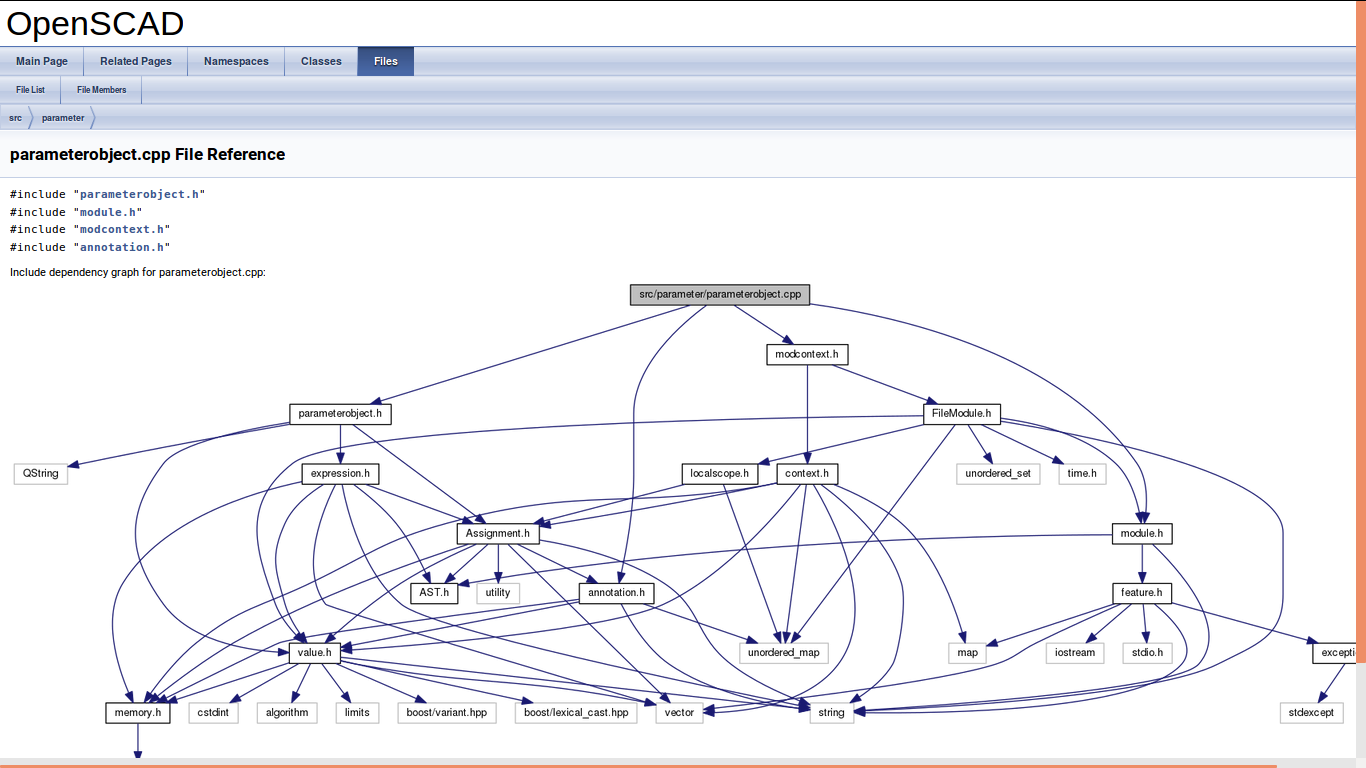
\includegraphics[scale=.35]{images/doc.png}
\caption{Documentation using Doxygen (main page)}
\end{figure}


\begin{figure}[H]
\centering 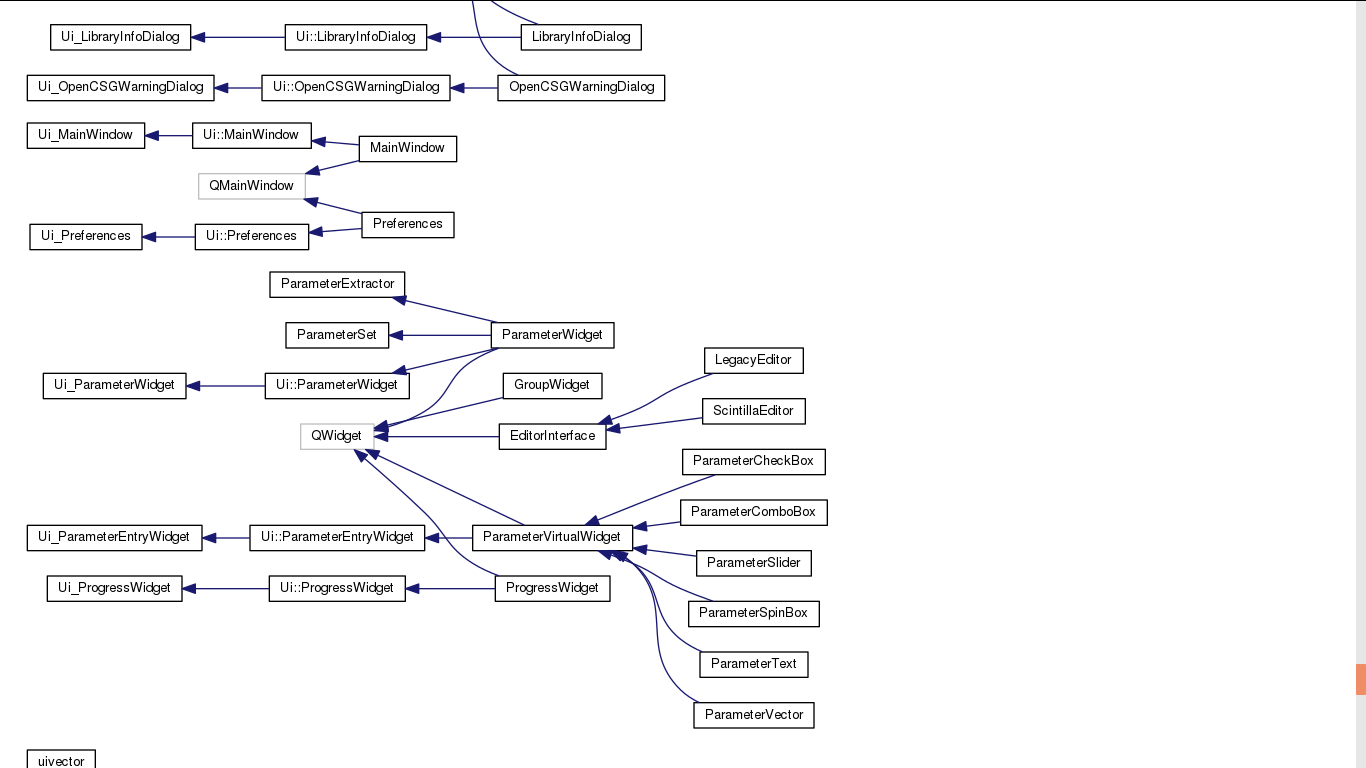
\includegraphics[scale=.35]{images/doc1.png}
\caption{Doxygen documentation of a function}
\end{figure}
\begin{figure}[H]
\centering 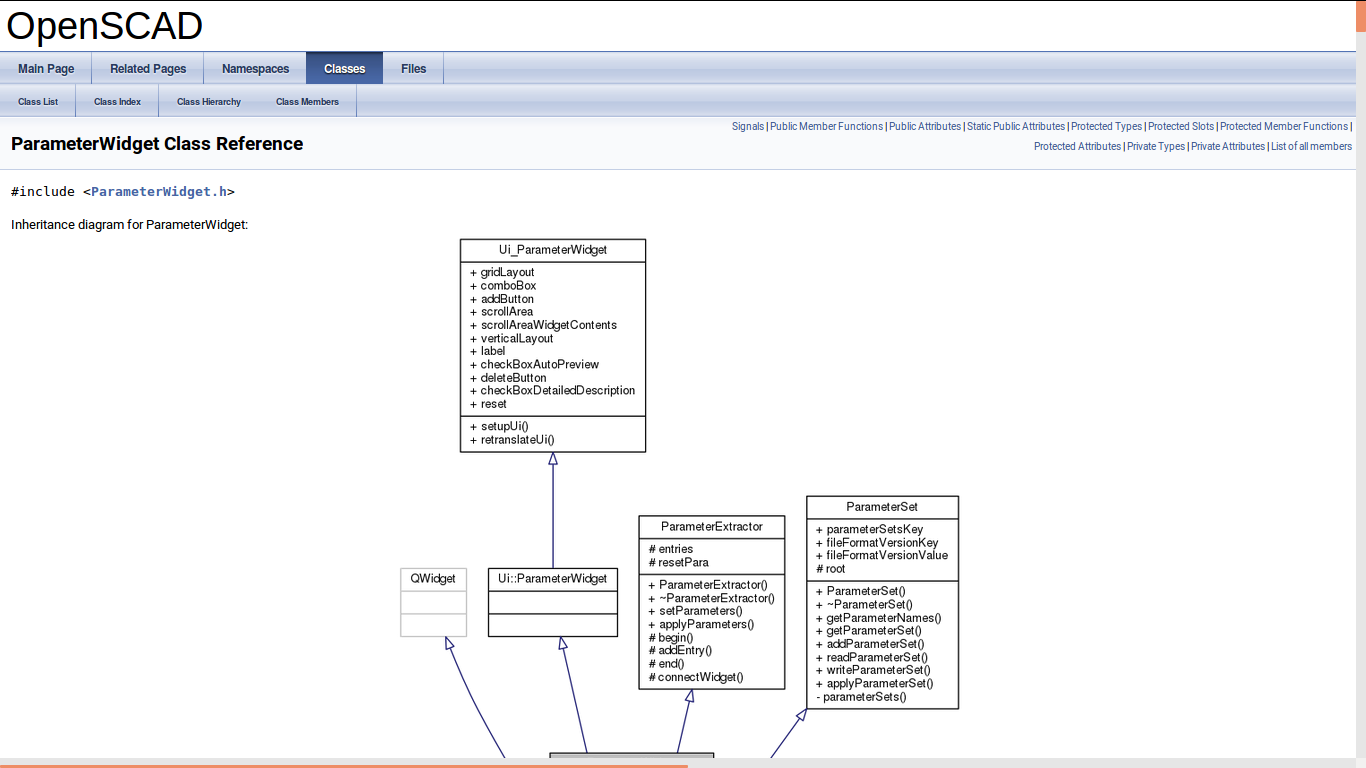
\includegraphics[scale=.35]{images/doc2.png}
\caption{Documentation using Doxygen(list of files)}
\end{figure}




\section{Introduction to Github}
\begin{figure}[!ht]
\centering

\includegraphics[width=0.3\textwidth]{images/github.png}                   
\caption{Github Logo}
\hspace{-1.5em}
\end{figure}
\leavevmode\\
GitHub is a Git repository web-based hosting service which offers all of the functionality of Git as well as adding many of its own features. Unlike Git which is strictly a command-line tool, Github provides a web-based graphical interface and desktop as well as mobile integration. It also provides access control and several collaboration features such as wikis, task management, and bug tracking and feature requests for every project.\\

GitHub has become such a staple amongst the open-source development community that many developers have begun considering it a replacement for a conventional resume and some employers require applications to provide a link to and have an active contributing GitHub account in order to qualify for a job.\\

The Git feature that really makes it stand apart from nearly every
other Source Code Management (SCM) out there is its branching model.\\
\\
Git allows and encourages you to have multiple local branches that can
be entirely independent of each other. The creation, merging, and
deletion of those lines of development takes seconds.\\ \\
This means that you can do things like:
\begin{itemize}
\item Frictionless Context Switching.\\ Create a branch to try out an
idea, commit a few times, switch back to where you branched from,
apply a patch, switch back to where you are experimenting, and merge
it in.
\item Role-Based Code lines. \\ Have a branch that always contains only
what goes to production, another that you merge work into for testing,
and several smaller ones for day to day work.
\item Feature Based Work flow. \\ Create new branches for each new
feature you're working on so you can seamlessly switch back and forth
between them, then delete each branch when that feature gets merged
into your main line.
\item Disposable Experimentation.\\  Create a branch to experiment in,
realize it's not going to work, and just delete it - abandoning the
work—with nobody else ever seeing it (even if you've pushed other
branches in the meantime).
\end{itemize}
Notably, when you push to a remote repository, you do not have to push
all of your branches. You can choose to share just one of your
branches, a few of them, or all of them. This tends to free people to
try new ideas without worrying about having to plan how and when they
are going to merge it in or share it with others.\\ \\
There are ways to accomplish some of this with other systems, but the
work involved is much more difficult and error-prone. Git makes this
process incredibly easy and it changes the way most developers work
when they learn it.

\subsection{What is Git?}
\begin{figure}[!ht]
\centering

\includegraphics[width=0.3\textwidth]{images/git.png}                   
\caption{Git Logo}
\hspace{-1.5em}
\end{figure}
Git is a distributed revision control and source code management (SCM) system with an emphasis on speed, data integrity, and support for distributed, non-linear workflows. Git was initially designed and developed by Linus Torvalds for Linux kernel development in 2005, and has since become the most widely adopted version control system for software development.\\

As with most other distributed revision control systems, and unlike most client–server systems, every Git working directory is a full-fledged repository with complete history and full version-tracking capabilities, independent of network access or a central server. Like the Linux kernel, Git is free and open source software distributed under the terms of the GNU General Public License version 2 to handle everything from small to very large projects with speed and efficiency.\\

Git is easy to learn and has a tiny footprint with lightning fast performance. It outclasses SCM tools like Subversion, CVS, Perforce, and ClearCase with features like cheap local branching, convenient staging areas, and multiple workflows.\\


\subsection{Various Git Commands}

Git is the open source distributed version control system that facilitates GitHub activities on your laptop or desktop. The commonly used Git command line instructions are:-\\

\begin{description}

\item [\$ git init [ project-name]]\\
Creates a new local repository with the specified name
\item [\$ git clone [url]]\\
Downloads a project and its entire version history\\
\item [\$ git merge [bookmark]/[branch]]\\
Combines bookmark’s branch into current local branch

\item [\$ git push [alias][branch]]\\
Uploads all local branch commits to GitHub

\item [\$ git pull] \leavevmode \\
Downloads bookmark history and incorporates changes

\item [\$ git add [file]]\\
Snapshots the file in preparation for versioning

\item [\$ git reset [file]]\\
Unstages the file, but preserve its contents

\item [\$ git commit -m "[descriptive message]"]\\
Records file snapshots permanently in version history\\

\end{description}
\section{Implementation}
\begin{figure}[H]
    \centering 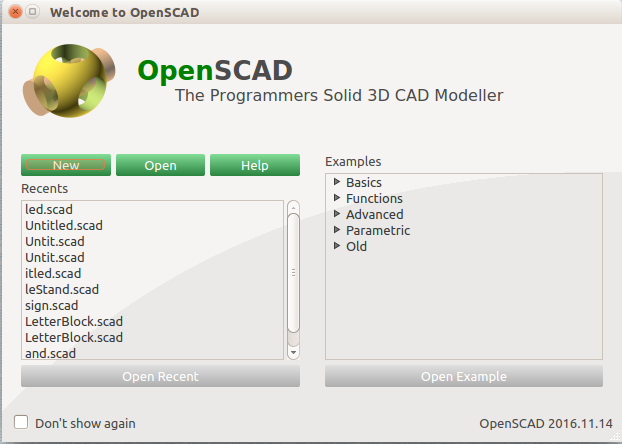
\includegraphics[width=0.7\linewidth]{images/output/1.png}
    \caption{StartUp Screen for OpenSCAD}
    \label{fig:1}
\end{figure}
\subsection{Multithreading}
In order to understand how we have attempted to implement multithreading for geometric rendering we need to understand the problem in substantial detail.\\
Even though it has been mentioned before profoundly, we feel the need the reiteration of what OpenSCAD is and how it achieves its goals. OpenSCAD is a 3D modeler i.e. it creates 3D models. The user interaction is done through a scripting language. This language describes the object(s) that the user wishes to create. This system has been put in place for the following reasons:
\begin{itemize}
	\item The fundamental geometric constructs of general purpose programming languages are too complex for an avergae computer user to learn and master. Even though ultimately, these constructs are being used to make everything in OpenSCAD but it is very difficult to expose the user to such tools. They are a little too fundamental and esoteric for the software to be of any help to your average modeler or designer who are unlikely to have much expertise of computer programming.\\
	That is why it becomes very important that the user is given an interface which has much less steeper learning curve than direct usage of geometric libraries. The OpenSCAD modelling language is just the interface for the job.
	\item Freedom and flexibilty of designing can be greatly compromised if only GUI constructs are used for modelling purpose. It is essential to give the user enough power to create complex and intricate designs easily without havnig to be limited by what the GUI has to offer. The modelling language, while being very intuitive is in fact very powerfull. The learning curve is much more user friendly without compromising the user's ability to make powerful designs. It saves a lot of time to use a higher abstraction of geometric constructs than to use the fundamentals them selves.\\
	The OpenSCAD modelling language thrives for the reasons any high level language thrives over a more machine related language. Time and effort of the programmer is saved and readability, portability are gained.
\end{itemize}
Here is a snapshot of the a model description using the above mentioned langauage:
\begin{figure}
    \centering 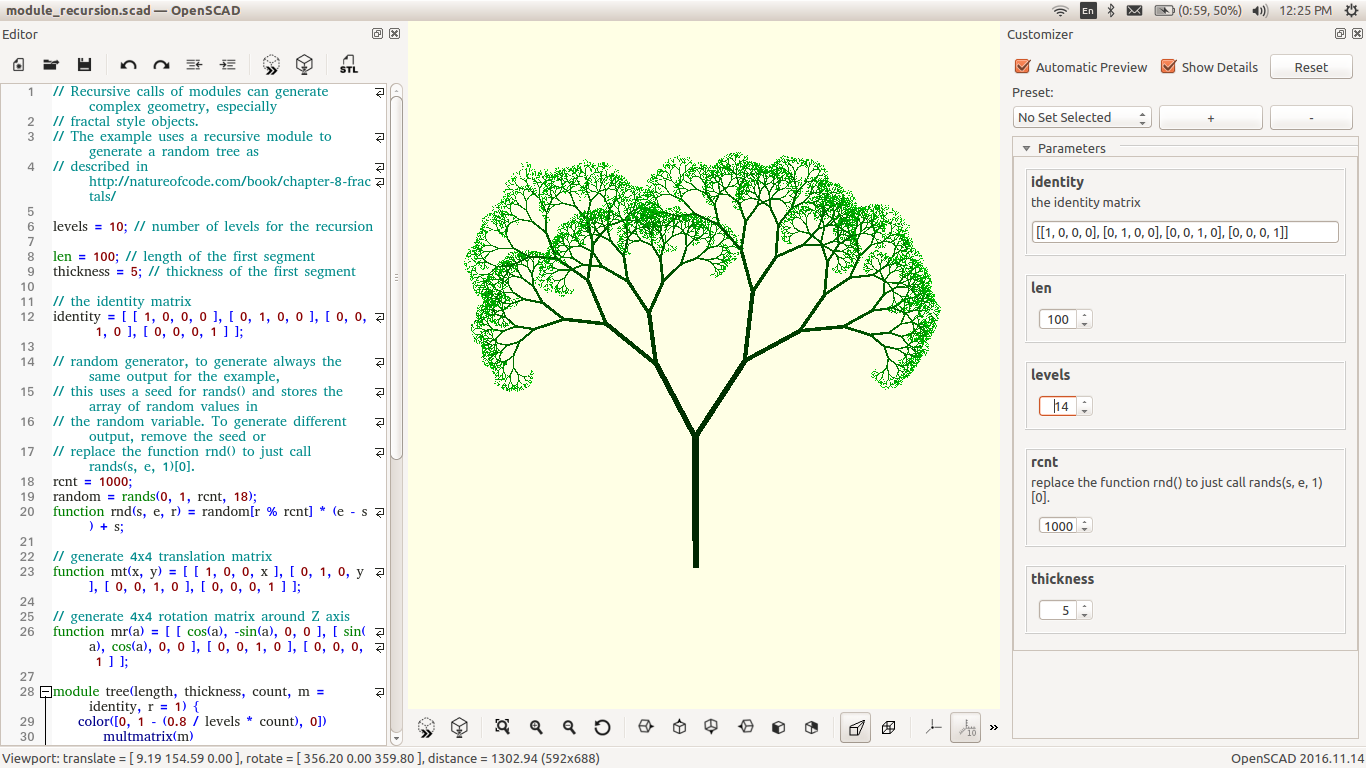
\includegraphics[width=\linewidth]{images/output/5.png}
    \caption{Working example of OpenSCAD}
    \label{fig:1}
\end{figure}
This language is parsed and converted into an Abstract Syntax Tree. This AST is used to turn descriptions of the objects into their graphic form. The AST is fed to an evaluator which reads the entire abstract syntac tree and turn it into a nodal tree. Each node in the tree represents geometric forms to be drawn. Once the node tree has been generated, references of this are pased around in order to accomplish various things. The same node tree can be used to generate the preview of the model using CSG and the same node tree is used to render the model. All of this can be summarised by the following flow chart:
\begin{figure}
    \centering 
    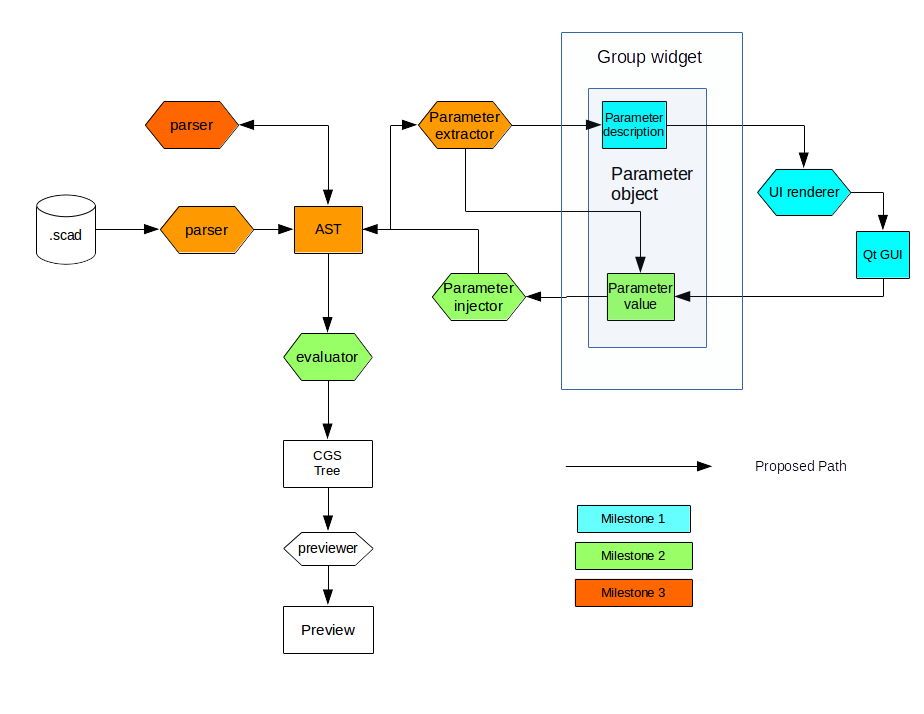
\includegraphics[width=\linewidth]{images/flowchart.png}
    \caption{Working flow of OpenSCAD}
\end{figure}
The first thing that was needed to be done was understanding the flow of the software and figuring out what sections of code needs to be parallelized. After forming a firmer understanding of the problem, it was required to check all the relevant data structures involved in evaluating the tree nodes. It was also be checked if any data structures used were needed to be modified or not. After fixing the appropriate data structures, all the feasible and plausible approaches were to be explored. Each approach has been evaluated on its merits and feasibility. Among all the options the one which is works well across all platform has been chosen. It goes without saying that the chosen solution has to meet all the requirement and implement the solution efficiently. After going through all of this the implementation began. The diagram below depicts the intended approach:
\begin{figure}
    \centering 
    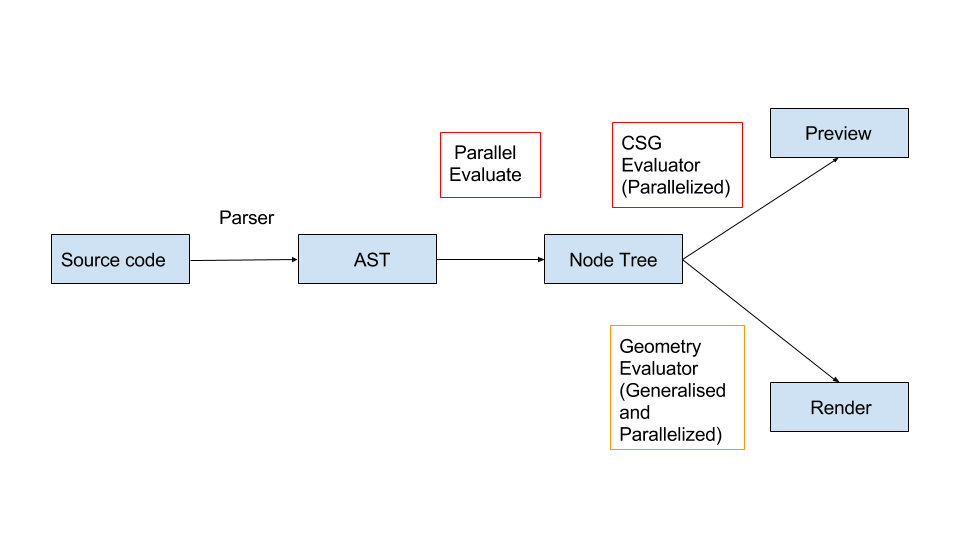
\includegraphics[width=\linewidth]{images/finalflow.png}
    \caption{Flowchart for the solution}
\end{figure}
During the implementation it was important to understand how the code works otherwise it will not have been possible to alter that code or even add to it. As OpenSCAD's GUI opens up, the code in the MainWindow.cc file is run. From here, the user can do many things but for our intent we are only going to focus on what happens when F6 is pressed. F6 is to issue the render command which is carried out via the actionRender() function. Following the flow of code from this function, it was descovered that the node tree is getting traversed recursively using the traverse function defined in the nodeVisitor.cc file. As mentioned, this function traverses each node is the node tree starting from the root node and then visiting each node recursively. Together with visiting each node, this function also calls out the accept() function on each node which is used to process the node further.\\
The whole point of multithreading was to parallelise this process of evaluating nodes. In its fundamental form, this is problem of applying parralelism to tree traversal. This parralelism can be achieved by simplying creating a new thread each time a new branch of the tree is to be traversed. But one may see, that this approach is not thread safe. First of all, the nodes that are getting visited must be accounted for in some sort of collection. And if various threads are going to visit the nodes and then update this collection then it becomes very important to make sure that no two threds are ever in a race, competing to update the collection at the same time. Such safety can be achieved by using lock mechanism.\\
This is not even the major problem, the real issue is in making sure that the global resources used by these functions are not unsafe from race conditions or concurrent access. Dealing with this took great effort and careful programming.
\subsection{Halting Mechanism for Render}
Ones the render process has been started, intentionally or unintentionally, there is nothing that can be done to stop the process without closing openSCAD altogether. The rendering process is not instantaneous making this a certain problem. There has to be method that on the user's command can halt an ongoing render process.\\
It is not just that the rendering process is to be stopped, it is also important to somehow perserve the partial work that has been done the rendering process before being halted by the user. This is achieved by caching the work and keeping the cache accesible across compiles in ordet to save time.\\
On carefull examination of the code, it was found that the cancel button was already part of the GUI. It just wasn't doing much usefull stuff to cancel the process. The cancel button is part of the progress widget GUI. And it is required to do is set a boolean variable to true. The variable name is wasCancelled. There is also function that checks the value of this variable to tell whether the process was cancelled or not i.e. the button was pressed or not. This function name is wasCancelled().\\
It is easy see that most pieces of the puzzle are already there. It is just required to place them properly and make them come together.\\
On some rigorous source browsing and consultation with the OpenSCAD developers, it was found that the assignment to true of the variable wasCancelled actually throws a programmer made exception: ProgressCancelException. Our job was to ensure that proper action is taken when this exception is raised. To do so, we had to tweak the visit() function which is responsible for visiting each node in the tree. This function was not singular. There were any overloaded versions of this depending on the type of node being visited. Hence the same work had to be done for each node.\\
After visiting each node, a made to call to a reporting function was made to happen. This function basically communicates to the progress widget about the number of nodes visited by it. The progress bar ranges from 1 to 1000. But this is not the sole purpose of this function, it also check at the end whether the exception has been raised or not. If it finds the exception is raised, it sets in motion a sequence of function calls that lead to safe halt of the render process. The following figure shows the working of the progress report and the cancel button:
\begin{figure}
	\centering
	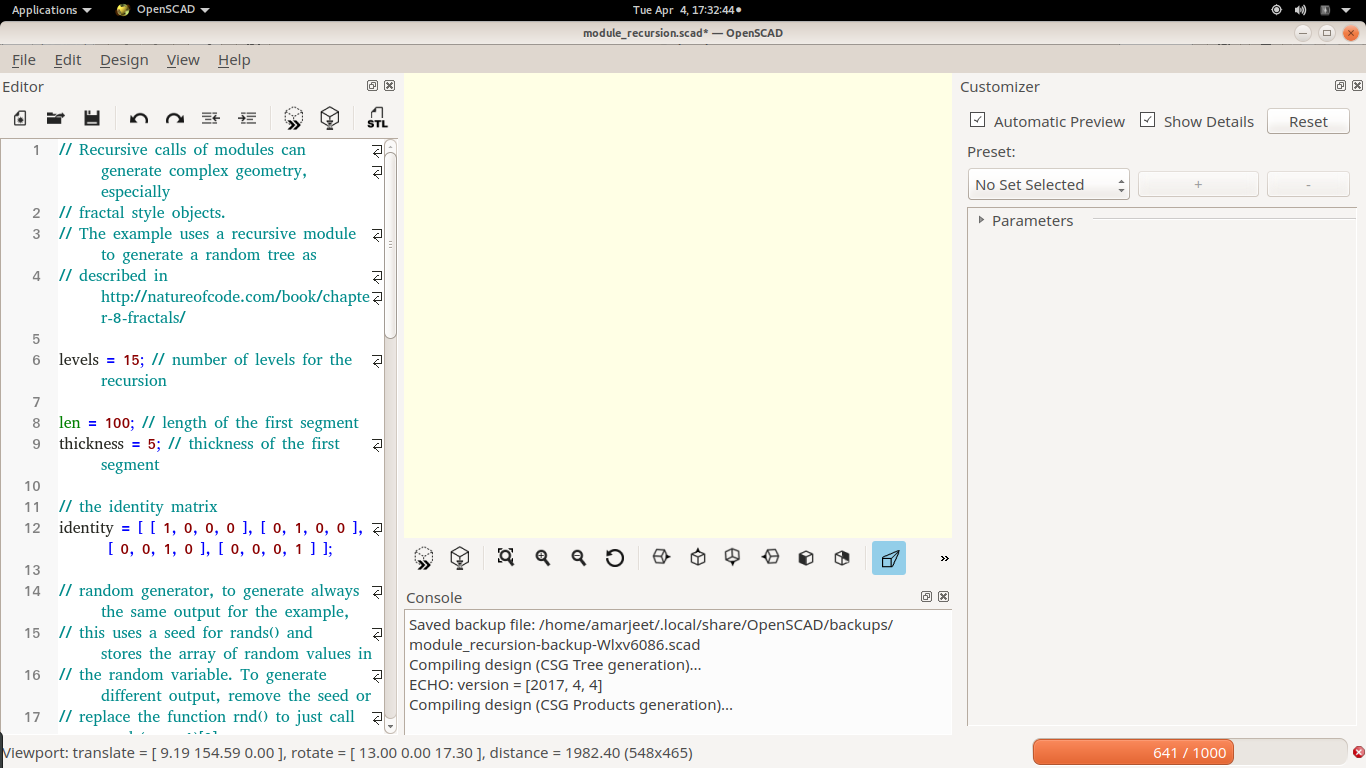
\includegraphics[width=\linewidth]{images/output/progress_widget.png}
	\caption{Progress Widget working}
\end{figure}
\subsection{Finding Root Tag Nodes}
3D models are often formed by taking two separate entities and then merging them using some of the operations like union, intersection and difference. All of this is taken care of at the back end using the node tree. In the node tree, one can have two separate entities as the child of a node and that node being the operation that is to be performed on those entities. As such, in the same model we can have various subsystem of nodes interacting with each other in order to give the final result. This just goes to show that subtrees within the node tree are very much capable of existing independantly. As such, sometimes it is desired by the user to only evaluate a certain branch of subtree of the whole tree. This means everything else in the tree except for that branch is useless for the time being. In order to save time and resources, we have to process and render only that subset.\\
The other parts of the tree are to be ignored. This certainly can not be done by commenting out, or deleting other nodes in the description of the language and then recompiling it. That approach would be very counterproductive.\\
A better way of doing this would be let the whole tree be in place. And when it is time to compile the part of the tree, simply tell the compiler to skip over to the subtree that is required and quit as soon as the compiler is done with that subtree. This way, nothing has to get deleted and only that part is compiled that is actually required. That is why there is a mechanism by which the user is allowed to set for a temporary period of time, a pseudo-root node. This root node can be anywhere in the tree. And when this is to be rendered, the software searches for it in the tree and returns a reference for it.\\
However, since the user is allowed to set multiple pseudo nodes in the tree, the searching function has to store references to all of them. Eventually only the first one of these stored references are used, but others are stored nonetheless. And if infact there are no such pseudo root nodes in the tree, then null is returned, indicating that the actuall root of the tree is to be treated as the root for the next render. It is important that we store all the nodes that have been marked as pseudo-roots. This marking is done by setting an attribute of each node to RootTag. This significanc stems from the fact that it is unnatural and hence useless to have multiple nodes as pseudo roots. For this reason, the user must be reminded as to how many markers have been set. This reminder is given in the form of a warning. In the picture below, one can see how the system worked before:\\
\begin{figure}
	\centering
	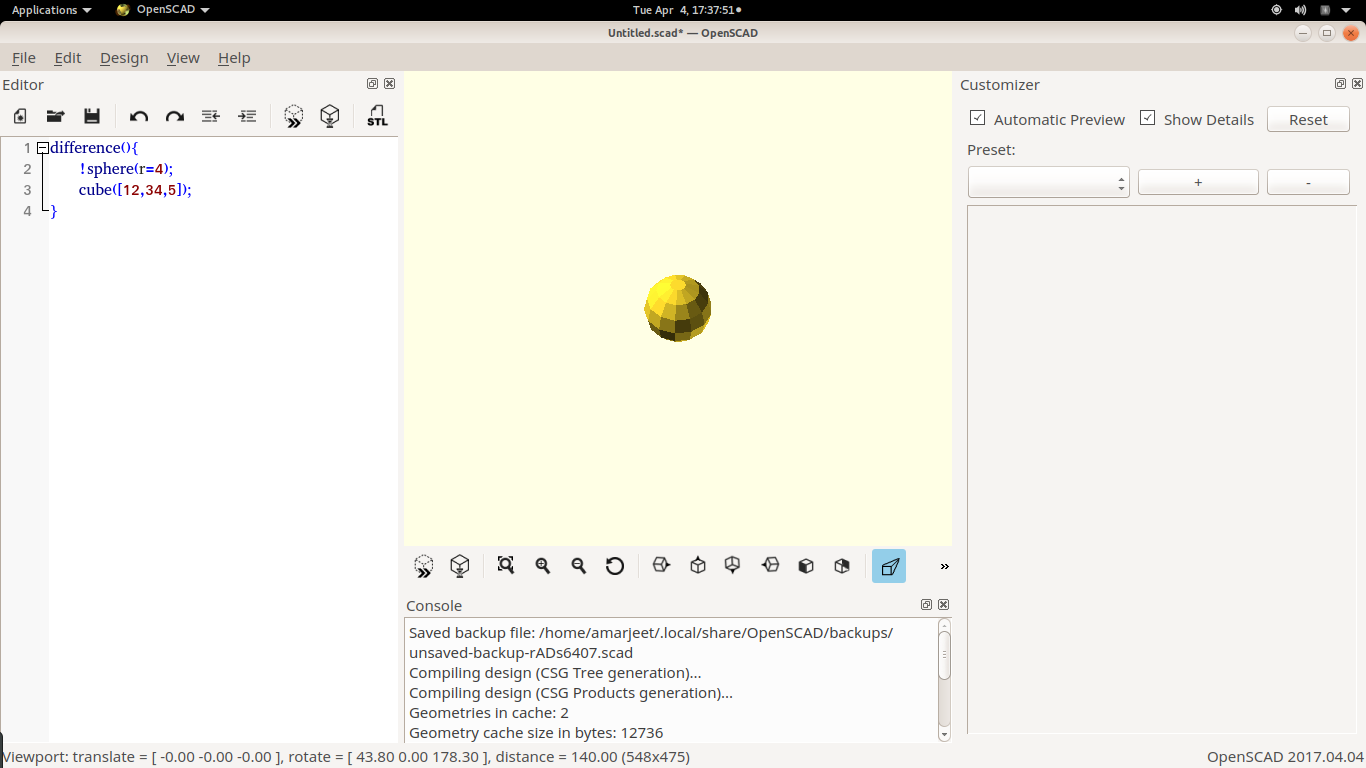
\includegraphics[width=\linewidth]{images/output/before_okay.png}
	\caption{Finding RootTag nodes previously}
\end{figure}
In this figure we can see how only one node has been marked as the pseudo root node (using the exclamation mark). And corresponding to it, we see no warnings because no warnings are due. But consider the following case:\\
\begin{figure}
	\centering
	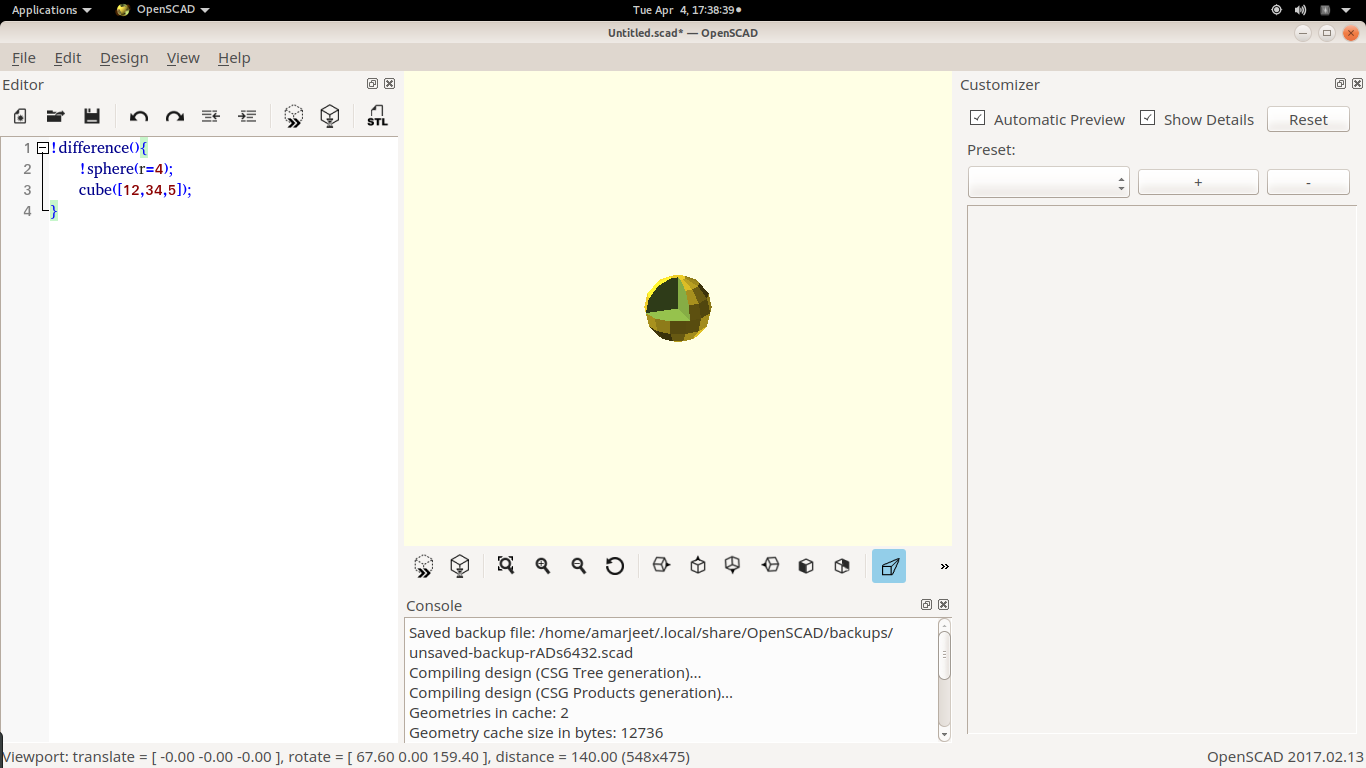
\includegraphics[width=\linewidth]{images/output/before_wrong.png}
	\caption{Finding multiple RootTag nodes previously}
\end{figure}
As seen, even though we had multilpe tags in the model, we didn't get any warnings.
The previous version of this function would search through the tree to find this tag. And the function would return as soon as it has found the first node with this tag or if it has exhausted the search space. In anycase, it was not possible to store all the nodes. We have implemented a solution to this problem by amending this search function.\\
In the present version of this function, we have implemented a lambda function. This lambda function recurses through the entire tree and checks to see if a node is marked or not. All the marked nodes are stored in vector. The result will still be the same as before because only the first element stored in the vector will be rendered, but atleast with this approach, the user is provided with a list of nodes that they have marked unnecessairily. The following figure shows how things are done now:\\
\begin{figure}
	\centering
	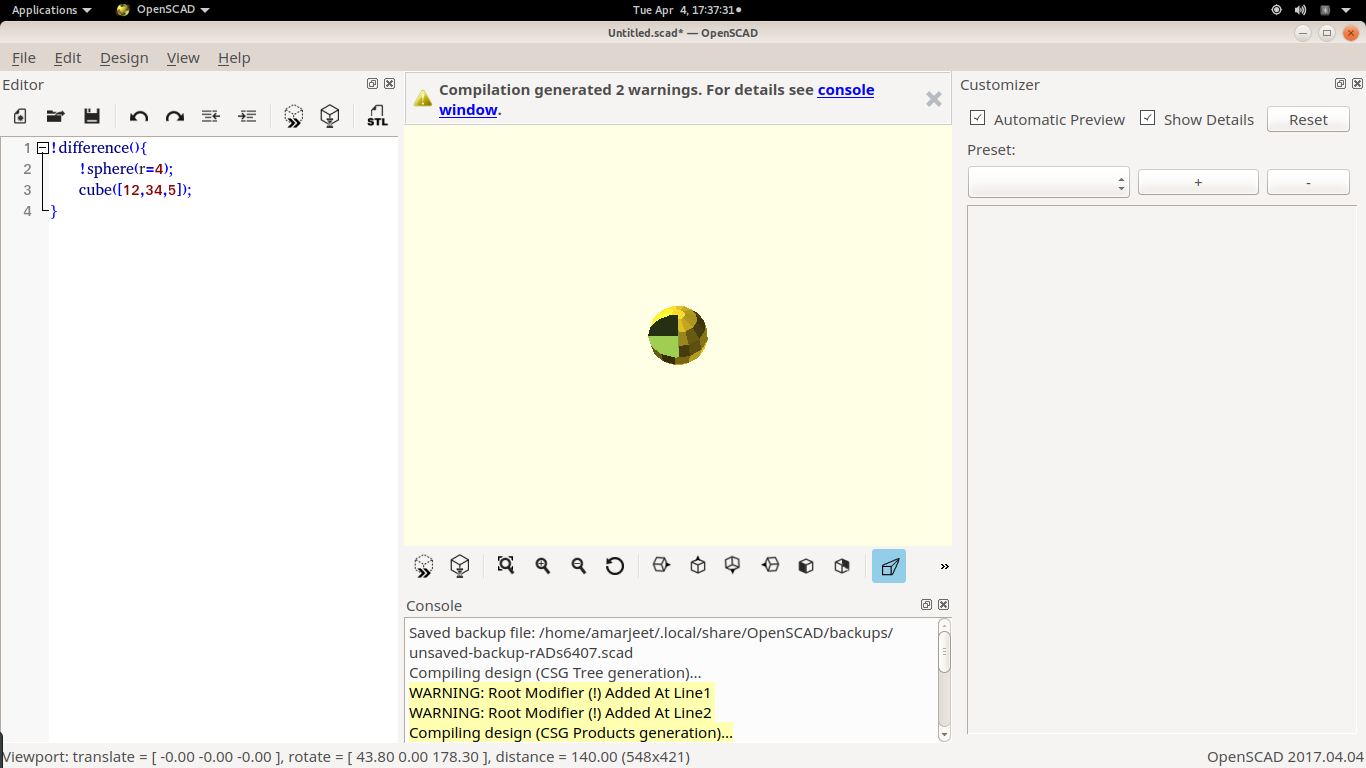
\includegraphics[width=\linewidth]{images/output/now_right.png}
	\caption{Finding multiple RootTag nodes now}
\end{figure}

\section{Testing}
\begin{figure}
    \centering
    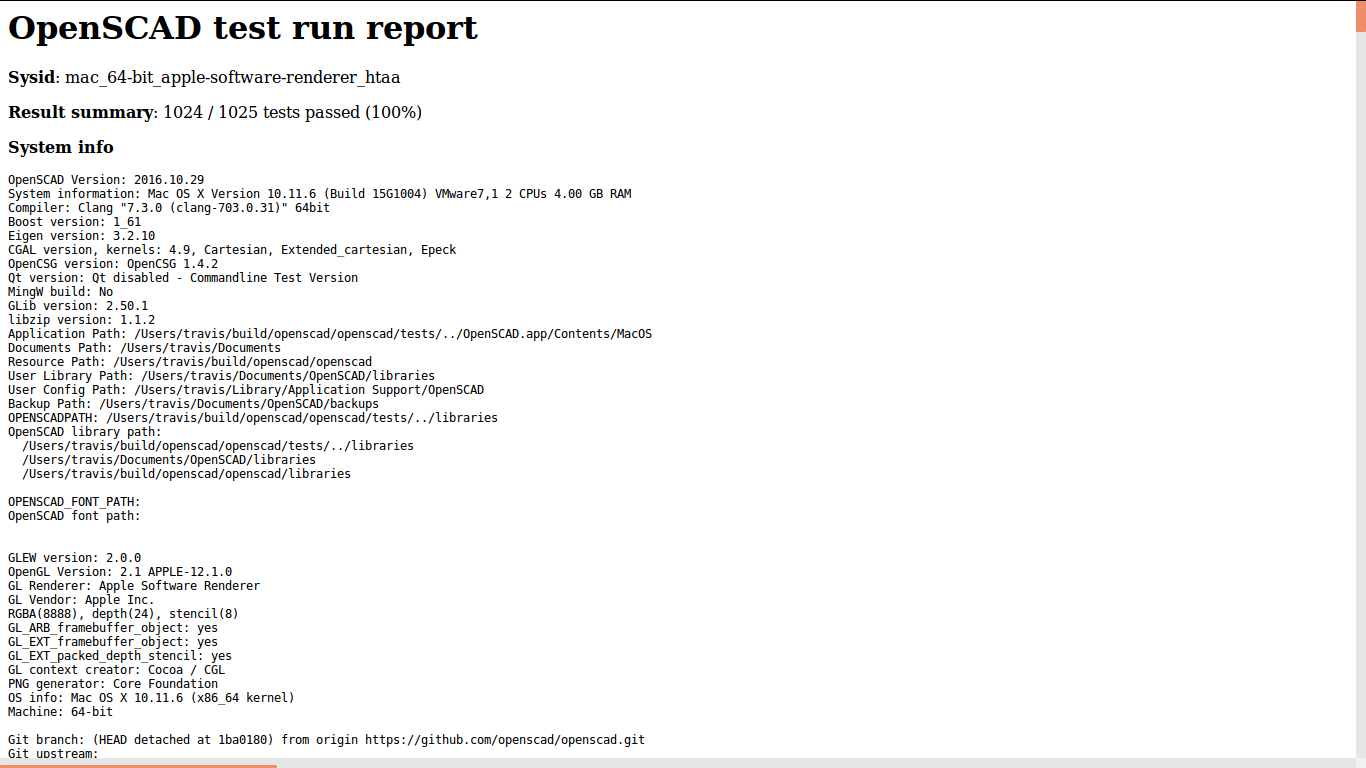
\includegraphics[width=\linewidth]{images/travisTestReport}
    \caption{Test Report by travis}
    \label{fig:travisTestReport}
\end{figure}

OpenSCAD is the software used by many of people all over the world and many web services as backend. so, it has to be perfect, Robust, reliable and bug-free. So, A very strong test suite is developed for testing this software and any component or feature that is to be integrated into OpenSCAD. And our project was able to pass all the task before getting Integrated into OpenSCAD.

Test Suit for OpenSCAD is developed using following two software:

\begin{enumerate}
    \item \textbf{cTest:} CTest is a testing tool distributed as a part of CMake. It can be used to automate updating (using CVS for example), configuring, building, testing, performing memory checking, performing coverage, and submitting results to a CDash or Dart dashboard system.
    cTest is used by OpenSCAD for testing the OpenSCAD on the local system of developers and it performs black box and regression testing of the software.
   
    \item \textbf{Travis CI:} Travis CI is a hosted, distributed continuous integration service used to build and test software projects hosted on GitHub.Open source projects may be tested at no charge via travis-ci.org. Private projects may be tested at the same location on a fee basis.
    Travis CI is used mainly for Installation testing on different OS and It also perform  black box and regression testing on different operating systems.
   
\end{enumerate}

Test Suit developed for OpenSCAD perform following type of testing:
 
 \begin{enumerate}
     \item \textbf{Installation Testing:} It is done by building the OpenSCAD from scratch on totally fresh installation of different operating systems. \ref{fig:travis}
   
     \begin{figure}
         \centering
         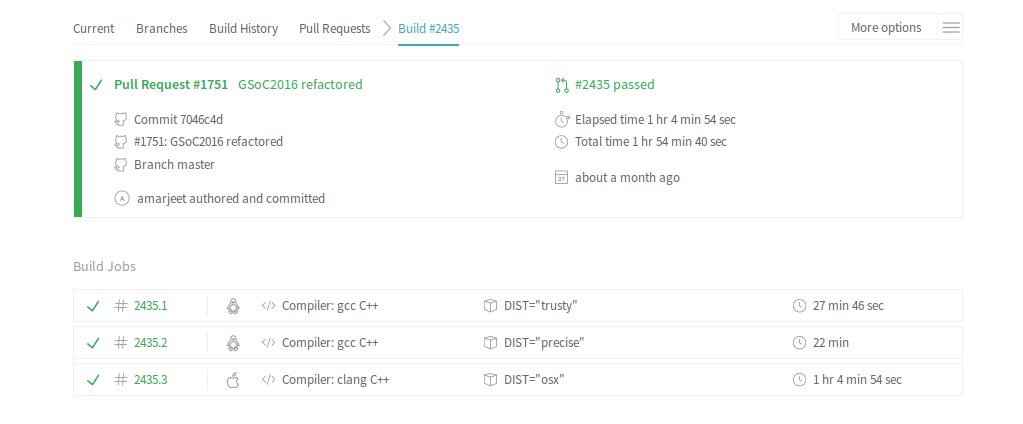
\includegraphics[width=\linewidth]{images/travis}
         \caption{Travis test summary for 3 different OS }
         \label{fig:travis}
     \end{figure}
   
     \item \textbf{Regression Testing:} It is done by running the test cases developed for the OpenSCAD before the New changes are made to check whether new Changes doesn't produce abnormal behavior. \ref{fig:generalTest}
   
     \begin{figure}
         \centering
         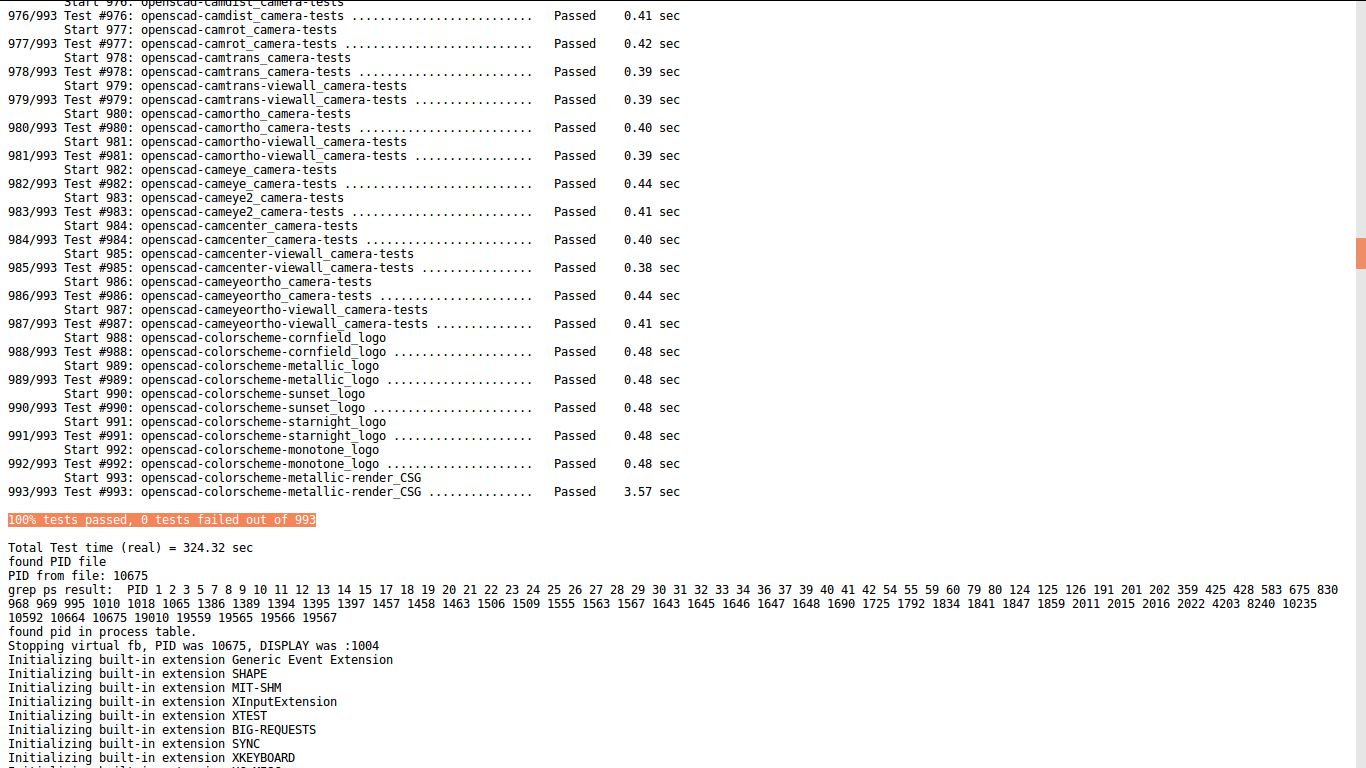
\includegraphics[width=\linewidth]{images/generalTest}
         \caption{Test whole software after Integration}
         \label{fig:generalTest}
     \end{figure}
   
     \item \textbf{Black Box Testing:} In this Testing, the for given set of input and the output is matched with the expected output. \ref{fig:ctest}
   
     \begin{figure}
         \centering
         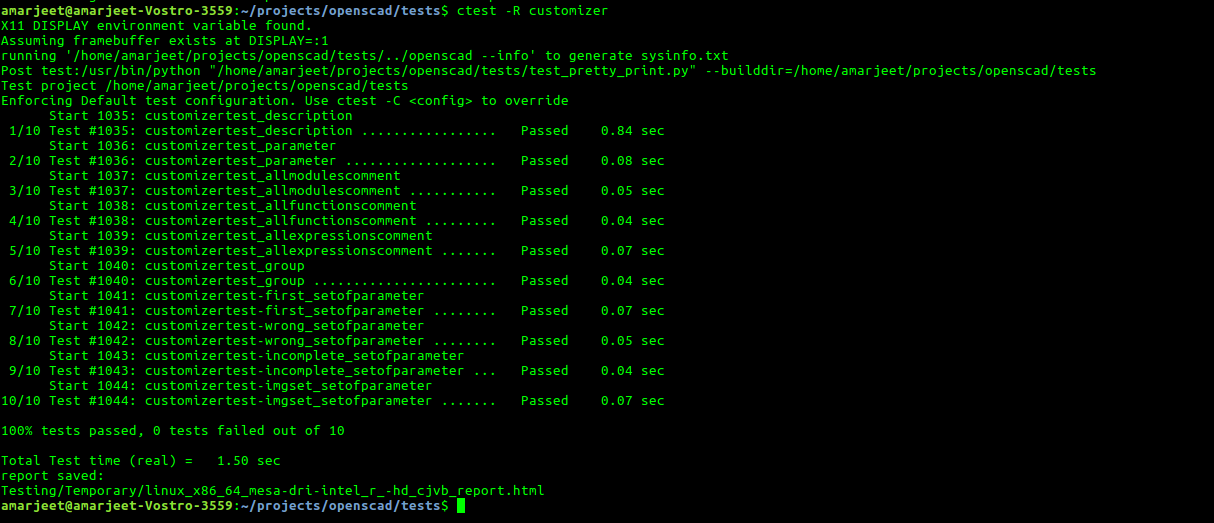
\includegraphics[width=\linewidth]{images/ctest}
         \caption{Tests on ctest}
         \label{fig:ctest}
     \end{figure}
   
 \end{enumerate}

\begin{figure}
    \centering
    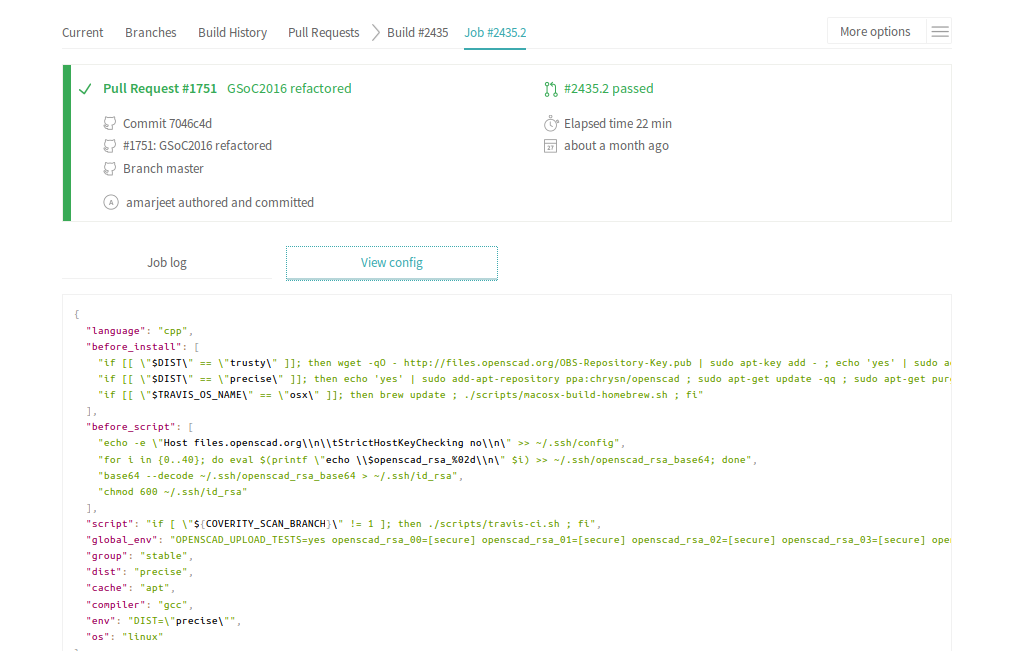
\includegraphics[width=\linewidth]{images/travisSpecific}
    \caption{Configuration and summary of single enviorment}
    \label{fig:travisSpecific}
\end{figure}
 
After passing above Test suit, our project went through system testing, which was of two types:
\begin{figure}
\centering
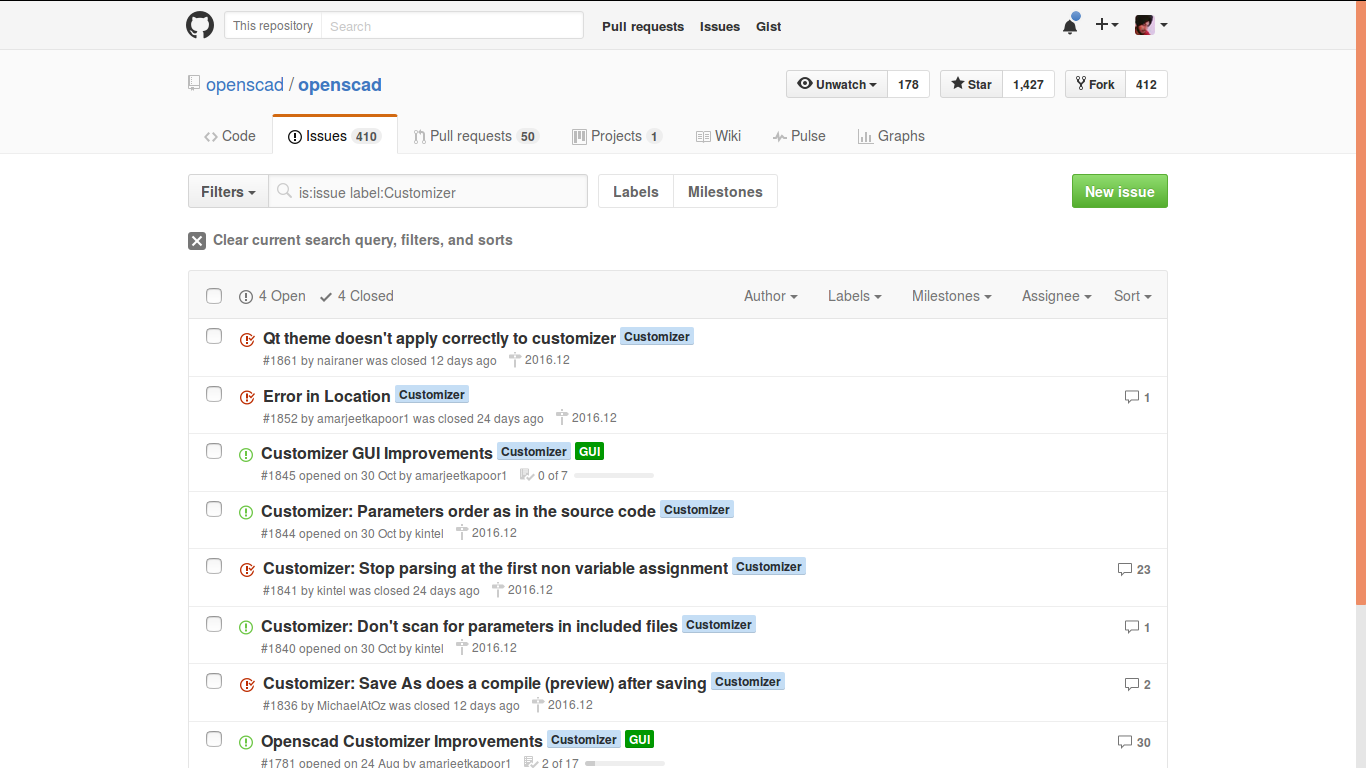
\includegraphics[width=\linewidth]{images/Issues}
\caption{List of Issues provide by Alpha and Beta testers}
\label{fig:Issues}
\end{figure}

\begin{enumerate}
    \item \textbf{Apha Testing}: In this our project was tested my fellow developers working for OpenSCAD community. The issues provided by them were improved and also Testing of User Interface was done. \ref{fig:Issues}
   
    \item \textbf{Beta Testing:} In this our project, was provided to community members and open to all people to test and report the issues or addition that are required to improve User Experience. \ref{fig:Issues}
   
\end{enumerate}

		
		


\chapter{CONCLUSION AND FUTURE SCOPE}
\section{Conclusion}
DoS is a very efficient application which help in generating result for analysis of structures. It
can be used by Civil Engineers and M.Tech. students and even layman. It's less time consuming and user-friendly which let the User work in batch mode 
and free him from all the installation process. It is a web application that can be accessed from a number of devices. The responsive User Interface makes it easy for the users to operate it. Many efforts were made to ease the usage for the users. Hence, it is expected to be work properly in different conditions. But any future bug reports or improvements are always welcomed and will be processed happily.

I learn a lot by working on this project. During this period I got to learn a vast number of
technologies. These are listed below:
Operating system: Ubuntu
Language used: Python, HTML, CSS, shellscript
Framework: Django
Technogloy: \LaTeX{}, Djanog, Doxygen, Sagemath, Git 
So during this project I learn  all the above things. Above all I got to know how software is
developed and how much work and attention to details is required in building even the most basic
of components of any project. Planning, designing, developing code, working in a team, testing,
etc. These are all very precious lessons in themselves.
Aside from all above I got go know about various methods like -:
\begin{enumerate}
\item Threading the programs 
\item Embedding and using different tech in one software.
\item How to work like in group for development of software.
\item How to apply juggaar(innovated) in softwares to get problem solved. 
\end{enumerate}

Beside these technology used in project I also get to know some other tech also like -:
\begin{enumerate}
\item  OpneCV (image processing)
\item opensshserver 
\item reveal.md, impress.js (for making presentations)
\end{enumerate}  



\section{Future Scope}
OpenSCAD being a open source project and supported by a large open Soure community have a lot of scope for future improvements and additions as other individuals can also contibute in it and add additional functionality. One of the example is my project only customizer for OpenSCAD.

Being a Open Soucre project their is constant flow of suggestion and demands by people for additional functionality and improvment in exiting features.
Customizer being no expection constant flow of feature of suggestions and feature requests even before the start of development. Her is small list of the Features that would be added in near future.

\begin{enumerate}

\item \textbf{Adding support for InBuid syntax:} It was decided much at beginning of the project that this feature will be ported using a special syntax then relying on the comment based syntax. Discussion has been going on related to deciding the syntax for customizer.   

\item \textbf{Option to Add images:} It have been proposed that their should be feature to add images through customizer.  

\item \textbf{Option to Include files with Customizer:} This feature will help people change the include file with the help of Customizer which could provide feature which would be related to Run Time Polymorphism.

\item \textbf{Conditional display of Parmaeter is customizer:} Sometime people want to show different set of parmaters based on the chooses made by user before that parameter or sometime we just want to hide the parameters because of selection made by user in pervious parameter.

\item \textbf{Improving GUI part:} There have been some suggestions related to improving the GUI of the Customizer
https://github.com/openscad/openscad/issues/1845 . 
\item \textbf{Providing syntax to manuplate modules parameter:} This feature will help user pick a customizer version of the module using the customizer. They will be able to Customize the parameters of modules using and the Customizer than drag that in to the file to call it with customized parameter.
\end{enumerate} 

Apart from these features their are Some suggestion related to how existing feature would be improved to refer to that you can visit following: 

\begin{enumerate}
	\item https://github.com/openscad/openscad/issues/1844
	\item https://github.com/openscad/openscad/issues/1840
	\item https://github.com/openscad/openscad/issues/1781
	\item https://github.com/openscad/openscad/issues/722
\end{enumerate} 



\begin{thebibliography}{9}
\bibitem{} Dynamics of Structure(DoS), https://github.com/amarjeetkapoor1/CivilOctave
\bibitem{} \LaTeX{} https://www.sharelatex.com
\bibitem{} Sagemath www.sagemath.org/
\bibitem{} Django https://docs.djangoproject.com/
\bibitem{} Doxygen www.doxygen.org
\bibitem{} My Blog, https://amarjeetkapoor1.wordpress.com
\bibitem{} My Github Profile, https://github.com/amarjeetkapoor1
https://en.wikipedia.org/wiki/OpenSCAD
http://www.openscad.org/
http://customizer.makerbot.com/docs
https://amarjeetkapoor1.wordpress.com/2016/07/04/user-interface-for-customizing-models/
%http://www.openscad.org/news.html#20160714


logo

https://www.quora.com/Is-there-an-official-C++-logo

%https://en.wikipedia.org/wiki/GNU#/media/File:Heckert_GNU_white.svg

%https://en.wikipedia.org/wiki/Qt_(software)#/media/File:Qt_logo_2015.svg

%https://upload.wikimedia.org/wikipedia/commons/c/ce/Doxygen.png

%https://en.wikipedia.org/wiki/GitHub#/media/File:GitHub_logo_2013_padded.svg

%https://en.wikipedia.org/wiki/Git#/media/File:Git-logo.svg

%Published by the Free Software Foundation
%51 Franklin Street, Fifth Floor
%Boston, MA 02110-1301 USA
%Printed copies are available from the Free Software Foundation.
%ISBN 1-882114-44-2

%https://en.wikipedia.org/wiki/Qt_(software)

%https://en.wikipedia.org/wiki/C%2B%2B

%Flex/Bison Tutorial
%Aaron Myles Landwehr
%aron+ta@udel.edu

\end{thebibliography}


\appendix
\chapter{Implementation Example}
Example 1: 
To Make Parameteric candle Stand model in OpenSCAD using customizer

\begin{figure}[H] 
	\centering 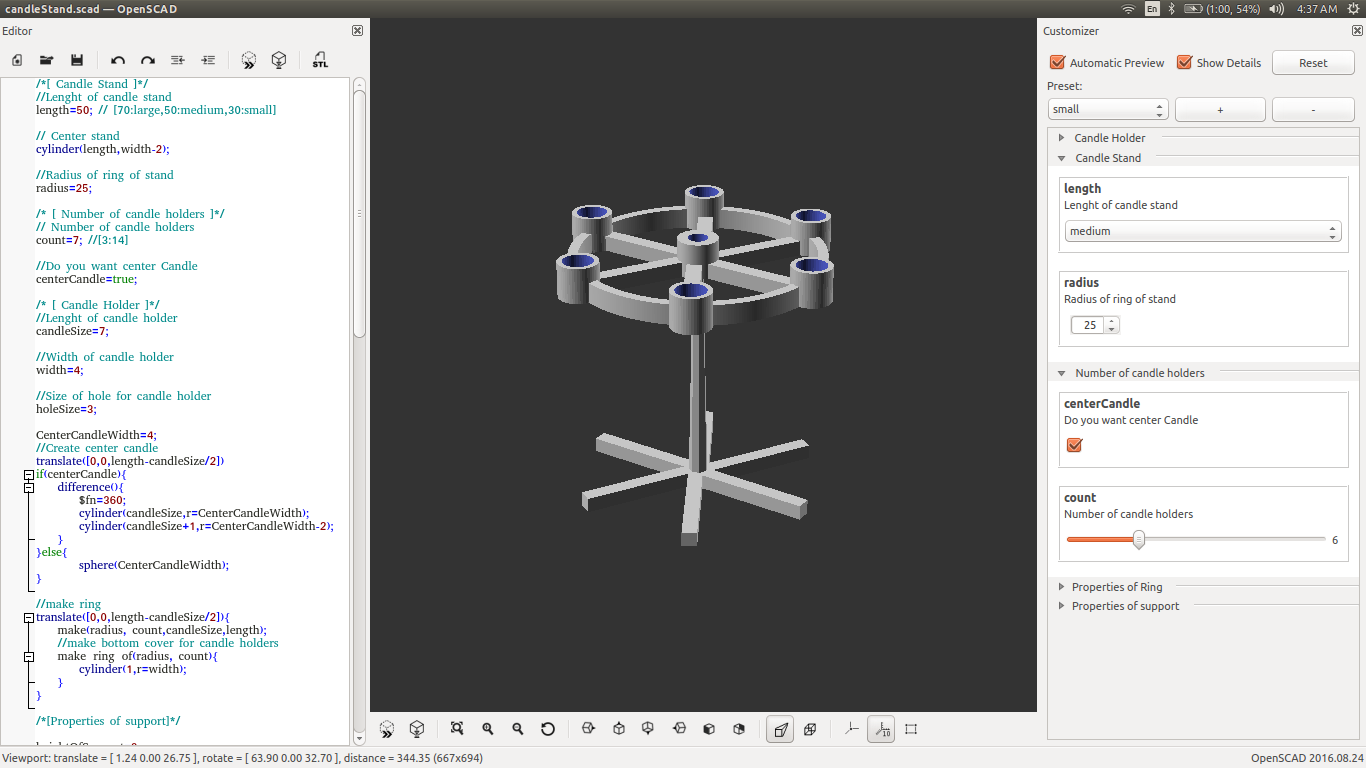
\includegraphics[scale=0.31]{images/output/9.png}
	\caption{Output of Code for Candle Stand model}
\end{figure}

\begin{lstlisting}[language=c++]
/*[ Candle Stand ]*/
//Lenght of candle stand
length=50; // [70:large,50:medium,30:small]

// Center stand
cylinder(length,width-2);

//Radius of ring of stand
radius=25;

/* [ Number of candle holders ]*/
// Number of candle holders
count=7; //[3:14]

//Do you want center Candle
centerCandle=true;

/* [ Candle Holder ]*/
//Lenght of candle holder
candleSize=7;

//Width of candle holder
width=4;

//Size of hole for candle holder
holeSize=3;

CenterCandleWidth=4;

/*[Properties of support]*/

heightOfSupport=3;
widthOfSupport=3;

/*[Properties of Ring]*/

heightOfRing=4;

widthOfRing=23;


//Create center candle
translate([0,0,length-candleSize/2])
if(centerCandle){
 difference(){
     $fn=360;
     cylinder(candleSize,r=CenterCandleWidth);
     cylinder(candleSize+1,r=CenterCandleWidth-2);
 }
}else{
     sphere(CenterCandleWidth);
}

//make ring 
translate([0,0,length-candleSize/2]){
 make(radius, count,candleSize,length);
 //make bottom cover for candle holders
 make_ring_of(radius, count){
     cylinder(1,r=width);
 }
}


//Base of candle stand
for (a = [0 : count - 1]) {
 rotate(a*360/count) {
 translate([0, -width/2, 0]) 
     cube([radius, widthOfSupport, heightOfSupport]);
 }
}

//make ring with candle holders
module make(radius, count,candleSize,length){
 
 $fa = 0.5;
 $fs = 0.5;
 difference(){
     union(){
          //making holders
         make_ring_of(radius, count){ 
             cylinder(candleSize,r=width);
         }
         
         //Attaching holders to stand
         for (a = [0 : count - 1]) {
             rotate(a*360/count) {
             translate([0, -width/2, 0]) 
                 cube([radius, widthOfSupport, heightOfSupport]);
             }
         }
         
         //make ring
         linear_extrude(heightOfRing)
         difference(){    
             circle(radius);
             circle(widthOfRing);
         }
     }
     //Making holes in candle holder
     make_ring_of(radius, count){
         cylinder(candleSize+1,r=holeSize);
     }
 }
}


module make_ring_of(radius, count){
 for (a = [0 : count - 1]) {
     angle = a * 360 / count;
     translate(radius * [cos(angle), -sin(angle), 0])
             children();
 }
}

// Written by Amarjeet Singh Kapoor <amarjeet.kapoor1@gmail.com>
//
// To the extent possible under law, the author(s) have dedicated all
// copyright and related and neighboring rights to this software to the
// public domain worldwide. This software is distributed without any
// warranty.
//
// You should have received a copy of the CC0 Public Domain
// Dedication along with this software.
// If not, see <http://creativecommons.org/publicdomain/zero/1.0/>.
\end{lstlisting}


\end{document}

